%% filename: amsbook-template.tex
%% version: 1.1
%% date: 2014/07/24
%%
%% American Mathematical Society
%% Technical Support
%% Publications Technical Group
%% 201 Charles Street
%% Providence, RI 02904
%% USA
%% tel: (401) 455-4080
%%      (800) 321-4267 (USA and Canada only)
%% fax: (401) 331-3842
%% email: tech-support@ams.org
%% 
%% Copyright 2006, 2008-2010, 2014 American Mathematical Society.
%% 
%% This work may be distributed and/or modified under the
%% conditions of the LaTeX Project Public License, either version 1.3c
%% of this license or (at your option) any later version.
%% The latest version of this license is in
%%   http://www.latex-project.org/lppl.txt
%% and version 1.3c or later is part of all distributions of LaTeX
%% version 2005/12/01 or later.
%% 
%% This work has the LPPL maintenance status `maintained'.
%% 
%% The Current Maintainer of this work is the American Mathematical
%% Society.
%%
%% ====================================================================

%    AMS-LaTeX v.2 driver file template for use with amsbook
%
%    Remove any commented or uncommented macros you do not use.

% TODO: Controllare se fa differenza su texstudio per lo spellcheck
% !TeX spellcheck = IT
\documentclass{amsbook}

%    For use when working on individual chapters
%    \includeonly{}

%    Include referenced packages here.

%    Font & encoding

\usepackage[utf8]{inputenc}
\usepackage[italian]{babel}
\usepackage[T1]{fontenc}

% 		Math 

\usepackage{amsthm, amsmath, amssymb, mathtools}
\usepackage{tikz-cd}    % TODO: non so se servirà, per ora l'ho messo.
\usepackage{derivative} % Serve: il comando che era dv è diventato odv

% 		Misc
\usepackage{hyperref}
\usepackage{booktabs}
\usepackage{dsfont}
% Note: se è possibile non usare il seguente package 
% \usepackage{mnsymbol} 

% Definition of sets and operators.
\def \Z {\mathbb{Z}}
\def \R {\mathbb{R}}
\def \C {\mathbb{C}}
\def \N {\mathbb{N}}
\def \S {\mathbb{S}}
\def \D {\mathbb{D}}
\def \Ind {\operatorname{Ind}}
\def \image {\operatorname{image}}

% Routine to write a general function given
% function name, domain and codomain.
\newcommand{\morphism}[3]{
	#1 \colon\ #2 \rightarrow #3
}
% Function diameter of a set
\newcommand{\diam}[1]{
	\operatorname{diam}\left(#1\right)
}
% Distance between two sets or a set and a point or whatever.
\newcommand{\dist}[2]{
	\operatorname{dist}\left(#1, #2\right)
}

% Theorems, definitions and styles 
\newtheorem{theorem}{Teorema}[chapter]
\newtheorem{lemma}[theorem]{Lemma}
\newtheorem{proposition}{Proposizione}[chapter]
\newtheorem{corollary}[theorem]{Corollario}

\theoremstyle{definition}
\newtheorem{definition}[theorem]{Definizione}
\newtheorem{example}[theorem]{Esempio}
\newtheorem{xca}[theorem]{Esercizio}

\theoremstyle{remark}
\newtheorem{remark}[theorem]{Osservazione}

\numberwithin{section}{chapter}
\numberwithin{equation}{chapter}

%    For a single index; for multiple indexes, see the manual
%    "Instructions for preparation of papers and monographs:
%    AMS-LaTeX" (instr-l.pdf in the AMS-LaTeX distribution).
\makeindex

\begin{document}

\frontmatter

\title{Analisi Complessa}

%    Remove any unused author tags.

% TODO: Decidere se mettere o meno i nomi
%    author one information
\author{A}
%    author two information
\author{B}
%    
\author{C}

% 
% \subjclass[2020]{}


\date{02/02/2020}

\begin{abstract}
	% TODO? 
\end{abstract}

\maketitle

%    Dedication.  If the dedication is longer than a line or two,
%    remove the centering instructions and the line break.
%\cleardoublepage
%\thispagestyle{empty}
%\vspace*{13.5pc}
%\begin{center}
%  Dedication text (use \\[2pt] for line break if necessary)
%\end{center}
%\cleardoublepage

%    Change page number to 6 if a dedication is present.
\setcounter{page}{4}

\tableofcontents

%    Include unnumbered chapters (preface, acknowledgments, etc.) here.
\chapter{Un dessert prima di pranzo}

Praticamente queste note seguiranno gli appunti delle lezioni di mezzo semestre dedicati all'analisi complessa del corso di laurea triennale di Trento a. s. il primo con il coronavirus e con l'introduzione dei mezzi digitali.
Sicché si dice che la matematica è un enorme battuta che nessuno capisce e poi va spiegata lentamente, 
queste note seguiranno lo stesso corso. Prima verranno introdotti alcuni teoremi che esprimeranno la bellezza di alcuni risultati 
e più avanti verranno motivati propriamente.

\section{Il meraviglioso complesso mondo}

Premessa di questa sezione è di mostrare alcune proprietà che rendono il campo complesso $\C$ magnifico e addirittura \textit{semplice}.

\begin{definition}
	Una \textbf{funzione olomorfa} è una funzione tale che $\morphism{f}{A \subset \C}{\C}$, dove $A$ aperto, differenziabile in senso complesso. 
\end{definition}

Ecco alcuni enunciati che semplificano la vita mentre si lavora con funzioni olomorfe in campo complesso.
\begin{theorem}[Integrazione lungo curve]
	Se $\alpha \sim \beta$ congiungono due punti di $A \subset \C$ allora 
	\begin{equation}
	\begin{aligned}
	\int_\alpha f = \int_\beta f
	\end{aligned}
	\end{equation}
\end{theorem}

\begin{theorem}[Regolarità]
	Se $f$ è olomorfa allora $f \in C^{\infty}(A)$ dove $A\subseteq \C$ è il dominio di $f$.
\end{theorem}

\begin{theorem}[Principio di identità]
	Sia $A\subset \C$ tale che $A \simeq \D$ per omotopie, allora se $f(x) = g(x)$ per ogni $x\in A$, allora $f = g$.
\end{theorem}


\mainmatter
%    Include main chapters here.

% Analisi complessa
\chapter{Calcolo differenziale}

\section{Differenziabilità in senso complesso}

Partiamo dal presupposto che possiamo indentificare $\C = \R^2$ dato che hanno la stessa topologia (e noi siamo interessati principalmente a questa struttura dato che vogliamo definire la contiuità e la differenziabilità in senso complesso). Per cui ogni funzione in una varabile complessa $\morphism{f}{\C}{\C}$ sarà essenzialmente trattata come se fosse una funzione $\morphism{f}{\R^2}{\R^2}$, ovvero ponendo $z = x + iy$
\begin{equation}
\begin{aligned}
	f(z) = u(x,y) + iv(x,y)
\end{aligned}
\end{equation}
ma bisogna ricordare che le proprietà di $i$ ci daranno delle condizioni ulteriori sui criteri per cui possiamo definire $u, v$ e quindi ciò che diremo sui complessi non si potrà estendere direttamente sulle funzione $\R^2 \to \R^2$. Intanto ricordiamo che $f$ è continua se e solo se $u,v$ lo sono (per proprietà universale del prodotto topologico).\\

Come nell'analisi reale in una variabile possiamo esprimere la differenziabilità in funzione del limite del rapporto incrementale

\begin{definition}
	Sia $z \in \Omega \subset \C$. La funzione $f$ si dice \textbf{differenziabile} se esiste un numero complesso $f'(z)$ tale che per $h \to 0$ vale la seguente relazione
	\begin{equation}
	\begin{aligned}
		f(z+ h) - f(z) = f'(z)h + o(|h|)
	\end{aligned}
	\end{equation} 
\end{definition}

\begin{definition}
	Sia $z \in \Omega \subset \C$. La \textbf{derivata direzionale} di $f$, se $f$ è differenziabile, lungo $v \in \C$ con $|v| = 1$, si definisce come
	\begin{equation}
	\begin{aligned}
		D_v f(z) = \lim_{r \to 0} \frac{f(z + rv) - f(z)}{r} = f'(z) v
	\end{aligned}
	\end{equation}
\end{definition}


Inoltre per come è stata definita la derivata tutte le proprietà che valgono in analisi reale in una variabile, valgono anche nel caso dell'analisi complessa. Quindi sarebbe interessante procedere con degli esempi, come la derivata delle seguenti funzioni (se sono differenziabili...)
\begin{equation}
\begin{aligned}
	f(z) = \log(|z|) \;\ f(z) = e^{iz - |z|} \;\ f(z) = (1 + i - z)z^2
\end{aligned}
\end{equation}
\\

Siccome ci interessa principalmente la questione della derivabilità proponiamo la seguente definizione

\begin{definition}
	Una funzione $\morphism{f}{\Omega \subset \C}{\C}$ è detta \textbf{olomorfa} se è differenziabile in ogni $z \in \Omega$. In generale indicheremo l'insieme delle funzioni olomorfe su $\Omega$ con $\mathcal{O}(\Omega)$.
\end{definition}

\begin{remark}
	Osserviamo inoltre che ogni funzione olomorfa è continua, basta rispolverare la dimostrazione fatta per l'analisi reale.
\end{remark}

In virtù della relazione stabilità precedentemente, ovvero che $f = u + iv$ per qualche $\morphism{u,v}{\R^2}{\R}$, otteniamo una condizione che ci eravamo limitati solo a `prevedere'.

\begin{theorem}[Equazioni di Cauchy-Riemann]
	Sia $f(x+iy) = u(x,y) + iv(x,y)$ una funzione complessa su $\Omega \subset \C$. Allora $f$ è differenziabile in $z \in \Omega$ se e solo se $u,v$ rispettano le seguenti condizioni in $z$: sono differenziabili e $u_x = v_y, u_y = - v_x$.
\end{theorem}
\begin{proof}[$\Rightarrow$]
	Supponiamo $f$ differenziabile in $z=x+iy$. Allora consideriamo le derivate direzionali lungo l'asse reale e quello immaginario
	\begin{equation}
	\begin{aligned}
		D_{1} f & = f'(z) = f_x(z) \\
		D_{i} f & = f'(z)i = f_y(z)
	\end{aligned}
	\end{equation}
	dove $f_x(z) = u_x(x,y) + iv_x(x,y)$ e $f_y(z) = u_y(x,y) + iv_y(x,y)$ da cui vale la relazione 
	\begin{equation}
	\begin{aligned}
		f'(z) = u_x(z) + iv_x(x,y) = -i(u_y(x,y) + iv_y(x,y))
	\end{aligned}
	\end{equation}	
	ovvero $u_x(x,y) = v_y(x,y), v_x(x,y) = -u_y(x,y)$. Inoltre ci serve osservare che $u,v$ sono differenziabili in $z$. Infatti valendo che $f$ è differenziabile, allora anche la sua parte reale è differenaziabile, come anche la sua parte immaginaria, e vale dunque per $h = a + ib$
	\begin{equation}
	\begin{aligned}
		u(z+h) - u(z) & = u_x a - v_x b + o(\sqrt{a^2 + b^2})\\
		v(z+h) - v(z) & = u_x b + v_x a + o(\sqrt{a^2 + b^2})
	\end{aligned}
	\end{equation}
	ovvero $u,v$ sono differenziabili in $z$ che era quanto si voleva dimostrare. 
\end{proof}
\begin{proof}[$\Leftarrow$]
	Supponiamo quindi che $u,v$ siano differenziabili in $z$ e valgano le relazioni sopra descritte. Allora facendo un po' di inverse-engegneriing rispetto all'ultimo punto si ottiene, sempre per $h = a + ib$
	\begin{equation}
	\begin{aligned}
		u(z+h) - u(z) & = a u_x(z) + b u_y(z) + o(|h|) = a u_x(z) - b v_x(z) + o(|h|) \\
		v(z+h) - v(z) & = a v_x(z) + b v_y(z) + o(|h|) = a v_x(z) + b u_x(z) + o(|h|) \\
		\end{aligned}
	\end{equation}
	da cui ricordando la definizione di $f$ si ottiene direttamente che $f$ è derivabile in senso complesso.
\end{proof}

\begin{corollary}
	La matrice delle funzioni reali $\morphism{(u,v)}{\Omega \subset \R^2}{\R^2}$ tali da descrivere una funzione complessa $f$, sono tali che  
	\begin{equation}
	\begin{aligned}
		J_{(u,v)} = \begin{array}{cc}
					u_x & - v_x\\
					v_x & u_x					
					\end{array}
	\end{aligned}
	\end{equation}
	e il determinante è $\det J_{(u,v)} = u^2_x + v^2_x \ge 0$.
\end{corollary}

\begin{corollary}
	Se $f'(z) = 0$ allora $f$ è una funzione costante.
\end{corollary}

\begin{corollary}
	Se $f = u + iv$ con $u(x,y) = r \in \R$ e $f \in C^1$, allora $0 = u_x = v_y$ e $0 = u_y = -v_x$ allora $f' = 0$ e dunque $f$ è una funzione costante. Viceversa se $v(x,y) = p \in \R$ allora $f$ è una funzione costante.   
\end{corollary}

\section{Funzioni armoniche, operatori di wirtinger}

\begin{definition}[Operatori di Wirtinger]
	Sia $\morphism{f}{\Omega}{\C}$ funzione di classe $C^1(\Omega)$. Allora possiamo definire i seguenti operatori
	\begin{equation}
	\begin{aligned}
		\frac{\partial f}{\partial z} := \frac{1}{2}(f_x - if_y) \quad\ \frac{\partial f}{\partial \overline{z}} := \frac{1}{2}(f_x + if_y)
	\end{aligned}
	\end{equation}
\end{definition}

\begin{remark}
	Si ottiene che una funzione soddisfa il teorema di Cauchy-Riemann sse vale 
	\begin{equation}
	\begin{aligned}
		\frac{\partial f}{\partial \overline{z}} = 0
	\end{aligned}
	\end{equation}
	inoltre se vale ciò (ovvero $f$ olomorfa) si ottiene che
	\begin{equation}
	\begin{aligned}
		\frac{\partial f(z)}{\partial z} = f'(z) 
	\end{aligned}
	\end{equation}
\end{remark}

\begin{remark}
	Se $f \in C^1(\Omega)$ allora soddisfa le equazioni di Cauchy-Riemann e in particolare se supponiamo ulteriormente derivabile la $f = u+iv$ (cosa che non è necessario supporre, dato che le funzioni olomorfe, come vederemo in seguito, sono $C^\infty$), possiamo notare una relazione sulle funzione $u,v$:
	\begin{equation}
	\begin{aligned}	
		u_{xx} & = (v_y)_x = (v_x)_y = (-u_y)_y = u_{yy} \\
		v_{xx} & = (-u_y)_x = -(u_x)_y = -(v_y)_y = -v_{yy}\\
	\end{aligned}
	\end{equation}
	ovvero le due funzioni reali sono \textbf{armoniche} dato che hanno laplaciano nullo. In generale vale il seguente enunciato che verrà dimostrato in seguito:\\
	
	\textit{Sia $\morphism{u}{\Omega \subset \R^2}{R}$ una funzione armonica su un dominio semplicemente connesso $\Omega$. Allora esiste una funzione armonica $\morphism{v}{\Omega}{\R}$ unica a meno di una costante tale che $f(z=x+iy) = u(x,y) + iv(x,y)$ sia una funzione olomorfa}.
\end{remark}		
	
\section{Funzioni analitiche o funzioni olomorfe?}

Il termine analitico si perde quando si incomincia a parlare di funzioni complesse dato che, come vedremo, l'insieme delle funzioni olomorfe coincide con quelle analitiche. Pertanto si preferisce descrivere le funzioni analitiche come funzioni olomorfe (che è una condizione facilmente accertabile, data anche l'equivalenza stabilità delle equazioni di Cauchy-Riemann). Per cui in questa sezione ci limitiamo a costruire la teoria base per stabilire la convergenza di serie complesse. Infine vedremo qualcosa il teorema di Abel che stabilisce un certo legame tra funzioni analitiche e olomorfe.\\

\begin{definition}
	\label{defn:successione-di-funzioni-complesse}
	Sia $\Omega \subset \C$ e sia $\{f_n\}_{n\in\N}$ con $\morphism{f_n}{\Omega}{\C}$ funzione, allora $\{f_n\}_{n\in\N}$ si dice \textbf{successione di funzioni complesse}.
\end{definition}

\begin{definition}
	\label{defn:serie-di-funzioni-complesse}
	Data una successione di funzioni complesse $\{f_n\}_{n\in\N}$ definite su $\Omega\subset\C$, allora 
	\begin{equation}
	\begin{aligned}
		\sum_{n=0}^{+\infty} f_n 
	\end{aligned}
	\end{equation}
	si dice \textbf{serie di funzioni complesse}.
\end{definition}

\begin{definition}
	\label{defn:convergenza-puntuale-successione}
	Data una successione di funzioni complesse definite su $\Omega$, $\{f_n\}_{n\in\N}$, se per ogni $z \in \Omega$ vale 
	\begin{equation}
	\begin{aligned}
		f_n(z) \to f(z) \quad\ \text{per}\ n \to +\infty
	\end{aligned}
	\end{equation}
	per una qualche $\morphism{f}{\Omega}{\C}$, allora si dice che la successione \textbf{converge puntualmente} a $f$.
\end{definition}

\begin{definition}
	\label{defn:convergenza-puntuale-serie}
	Data una successione di funzioni complesse definite su $\Omega$, $\{f_n\}_{n\in\N}$, se per ogni $z \in \Omega$ vale 
	\begin{equation}
	\begin{aligned}
		\sum^{n}_{k=0} f_k(z) \to f(z) \quad\ \text{per}\ n \to +\infty
	\end{aligned}
	\end{equation}
	per una qualche $\morphism{f}{\Omega}{\C}$, allora si dice che la serie \textbf{converge puntualmente} a $f$.
\end{definition}

\begin{definition}
	\label{defn:convergenza-uniforme-successione}
	Data una successione di funzioni complesse definite su $\Omega$, $\{f_n\}_{n\in\N}$, se vale 
	\begin{equation}
	\begin{aligned}
		\sup_{z \in \Omega} |f_n(z) - f(z)| \to 0 \quad\ \text{per}\ n \to +\infty
	\end{aligned}
	\end{equation}
	per una qualche $\morphism{f}{\Omega}{\C}$, allora si dice che la successione \textbf{converge uniformemente} a $f$.
\end{definition}

\begin{definition}
	\label{defn:convergenza-uniforme-serie}
	Data una successione di funzioni complesse definite su $\Omega$, $\{f_n\}_{n\in\N}$, se vale 
	\begin{equation}
	\begin{aligned}
		\sup_{z \in \Omega} |\sum^{N}_{n=0}f_n(z) - f(z)| \to 0 \quad\ \text{per}\ N \to +\infty
	\end{aligned}
	\end{equation}
	per una qualche $\morphism{f}{\Omega}{\C}$, allora si dice che la serie \textbf{converge uniformemente} a $f$.
\end{definition}	
	
\begin{definition}
	\label{defn:convergenza-assoluta}
	Data una successione di funzioni complesse definite su $\Omega$, $\{f_n\}_{n\in\N}$, se per ogni $z \in \Omega$ vale 
	\begin{equation}
	\begin{aligned}
		\sum^{+\infty}_{n=0} |f_n|(z) < +\infty \quad\ \text{per}\ n \to +\infty
	\end{aligned}
	\end{equation}
	allora si dice che la serie \textbf{converge assolutamente}.	
\end{definition}

\begin{remark}
	Osserviamo infine che se una serie $\{\sum^n_{k=0}f_k\}_{n \in \N}$ è assolutamente convergente, allora è anche puntualmente convergente, infatti
	\begin{equation}
	\begin{aligned}
		|\sum^n_{k=0} f_k(z)| \le \sum^n_{k=0} |f_k(z)| = l < +\infty
	\end{aligned}
	\end{equation} 
	per cui $\sum^n_{k=0} \Re(f_k(z)) < +\infty,\ \sum^n_{k=0} \Im(f_k(z)) < +\infty$. Per cui tutta la serie converge a qualche funzione $f$ in ogni punto.
\end{remark}

\begin{theorem}[M-test di Weierstrass]
	\label{thr:m-test-weierstrass} Sia $\{f_n\}_{n\in\N}$ una successione di funzioni complesse e $\{M_n\}_{n\in\N}$ una successione di numeri reali positivi per cui vale per ogni $z\in \Omega$, $|f_n(z)| \le M_n$. Se la serie 
	\begin{equation}
	\begin{aligned}
		\sum_{n=0}^{+\infty} M_n < +\infty
	\end{aligned}
	\end{equation} 
	allora anche la serie 
	\begin{equation}
	\begin{aligned}
		\sum_{n=0}^{+\infty} f_n(z)
	\end{aligned}
	\end{equation}
	converge assolutamente e uniformemente in $\Omega$.
\end{theorem}
\begin{proof}
	È ovvio che la serie converge assolutamente per ipotesi su tutto $\Omega$. Per cui definiamo $s_n(z) := \sum_{k=0}^n f_k(z)$ e sia $s$ la funzione a cui converge la serie. Allora
	\begin{equation}
	\begin{aligned}
		|s - s_n| = \left|\sum_{k=n+1}^{+\infty} f_k\right| \le \sum_{k=n+1}^{+\infty} \left|f_k\right| \le \sum_{k=n+1}^{+\infty} M_k
	\end{aligned}
	\end{equation}
	per cui, dato che la serie degli $M_k$ converge, fissato un qualsiasi $\varepsilon > 0$ possiamo sempre trovare $N$ tale per cui $\sum_{k>N} M_k < \varepsilon$ da cui la tesi di uniforme convergenza data l'assoluta generalità con cui è stato scelto $z \in \Omega$. 
\end{proof}

\begin{definition}
	\label{defn:serie-di-potenze}
	Siano $z_0 \in \C$ e una successione $\{a_n\}_{n\in \N}$ di valori in $\C$, allora si definisce \textbf{serie di potenze} le serie della seguente forma
	\begin{equation}
	\begin{aligned}
		S(z) := \sum_{n=0}^{+\infty} a_n(z-z_0)^n
	\end{aligned}
	\end{equation}
\end{definition}

\begin{theorem}[Criterio di Hadamard]
	\label{thr:criterio-hadamard}
	Data una serie di potenze $S$ con notazione come in Definizione \ref{defn:serie-di-potenze}, allora definiamo il \textbf{raggio di convergenza} $R := ( \limsup_{n\to+\infty} \sqrt[n]{a_n})^{-1} \in \left[0,+\infty\right]$. Allora 
	\begin{enumerate}
		\item La serie di potenze $S$ converge assolutamente nel disco $B_{z_0}(R)$ e non converge per $z \notin \overline{B_{z_0}(R)}$.
		\item La serie di potenze converge su ogni disco chiuso $\overline{B_{z_0}(r)}$ con $r < R$.  
	\end{enumerate}
\end{theorem}
\begin{proof}
	Possiamo supporre $z_0 = 0$ tanto non fa differenza, dato che basta fare una sostituzione per riportarci nel caso $z_0 = 0$ data una qualsiasi $z_0 \in \C$.\\ 
	Dimostro che la serie di potenze converge uniformemente e assolutamente per ogni $0 < r < R$. Essendo $R < t^{-1}$ allora esiste un $N$ per cui
	\begin{equation}
	\begin{aligned}
		\sqrt[n]{a_n} < t^{-1} \quad\ \text{per ogni}\ n \ge N 
	\end{aligned}
	\end{equation}
	dunque $|a_n| < t^{-n}$ per ogni $n \ge N$. Se $|z| \le r$ allora vale
	\begin{equation}
	\begin{aligned}
		|a_nz^n| < \left(\frac{r}{t}\right)^n
	\end{aligned}
	\end{equation}
	Per il Teorema \ref{thr:m-test-weierstrass} la serie di potenze converge per ogni $z \in \Omega$ dove $\Omega = B_0(r)$ e siccome vale per ogni $r < R$, allora segue che vale anche per $B_0(R)$.\\
	
	Dimostriamo ora che non converge da nessuna parte al di fuori della chiusura del disco aperto $\overline{B_{z_0}(R)}$. Infatti se supponessimo la convergenza in qualche punto $z \in \C \setminus \overline{B_{z_0}(R)}$ allora $|z| > R$ e $|z|^{-1} < R$. Per cui per ogni $n \ge N$ per qualche $N \in \N$ vale che
	\begin{equation}
	\begin{aligned}
		|z|^{-1} < \sqrt[n]{|a_n|}
	\end{aligned}
	\end{equation}
	per cui otteniamo che 
	\begin{equation}
	\begin{aligned}
		\sum^{+\infty}_{n=0}|z|^{-n}|z|^n = \sum^{+\infty}_{n=0}|\sqrt[n]{|a_n|}|^n|z|^n < \sum^{+\infty}_{n=0}|a_n||z^n| 
	\end{aligned}
	\end{equation}
	e la prima serie è ovviamente non assolutamente convergente per ogni $|z| > R$.
\end{proof}

\begin{theorem}
	\label{prop:invarianza-raggio-convergenza-derivata}
	Data una serie di potenze definiamo la sua derivata come 
	\begin{equation}
	\begin{aligned}
		S'(z) = \sum^{+\infty}_{k=1} ka_k(z-z_0)^{k-1}
	\end{aligned}
	\end{equation} 
	allora i raggi di convergenza di $S'$ e $S$ sono gli stessi.
\end{theorem}
\begin{proof}
	È un ovvia applicazione del calcolo dei limiti, definiamo con $b_n = (n+1)a_{n+1}$ i coefficienti della serie di potenze derivata. Allora 
	\begin{equation}
	\begin{aligned}
		\limsup_{n\to+\infty} \sqrt[n]{b_n} & = \limsup_{n\to+\infty} \sqrt[n]{(n+1)a_{n+1}} \\
											& = \limsup_{n\to+\infty} \sqrt[n]{(n+1)} \sqrt[n]{a_{n+1}} \\
											& = \limsup_{n\to+\infty} \sqrt[n]{a_{n+1}} = \limsup_{n\to+\infty} \sqrt[n]{a_{n}} 
	\end{aligned}
	\end{equation}
	che è appunto lo stesso raggio di convergenza.
\end{proof}

\begin{theorem}[Teorema di Abel]
	\label{thr:teorema-di-abel}
	Sia $S$ una serie di potenze con raggio di convergenza $R > 0$. Allora $S(z)$ è una funzione olomorfa in $|z-z_0| < R$ e $S'$ è la sua derivata.
\end{theorem}
\begin{proof}
	Assumiamo ancora una volta che $z_0$ della serie di potenze sia $z_0 = 0$. Prendiamo quindi $z \in B_0(R)$ e sia $\delta > 0$ tale che $\overline{B_0(\delta)} \subset B_0(R)$. Prendiamo quindi un $h \in B_0(\delta)$. Allora
	\begin{equation}
	\begin{aligned}
		\frac{f(z+h) - f(z)}{h} & = \sum^{+\infty}_{n=0} a_n \frac{(z+h)^n - z^n}{h} = \sum^{+\infty}_{n=0} a_n \frac{(z+h)^n-z^n}{z+h-z} \\
								& = \sum^{+\infty}_{n=0} a_n z^{n-1} \frac{\left(\frac{z+h}{z}\right)^n - 1}{\left(\frac{z+h}{z}\right)^n - 1} \\
								& = \sum^{+\infty}_{n=0} a_n \sum^{n-1}_{j=0} z^{n-1-j}(z+h)^j 
	\end{aligned}
	\end{equation}
	vogliamo mostrare che la serie sopra descritta converge uniformemente, infatti
	\begin{equation}
	\begin{aligned}
		|z+h| \le |z| + |h| \le |z| + \delta
	\end{aligned}
	\end{equation}
	e quindi possiamo scrivere 
	\begin{equation}
	\begin{aligned}
		\left|a_n \sum^{n-1}_{j=0} z^{n-1-j}(z+h)^j \right| \le n|a_n|(|z|+\delta)^{n-1} 
	\end{aligned}
	\end{equation}
	utilizzando il Teorema \ref{thr:m-test-weierstrass} con $M_n = n|a+n|(|z|+\delta)^{n-1}$ sappiamo che converge per ogni $|z|+\delta < R$ dato che dal Teorema \ref{prop:invarianza-raggio-convergenza-derivata} vale che la derivata di una funzione ha lo stesso raggio di convergenza della funzione stessa. Per cui sappiamo che converge uniformemente per ogni $|z| < R$. 
	Per cui possiamo calcolare il limite del rapporto incrementale, da cui si ottiene 
	\begin{equation}
	\begin{aligned}
		\lim_{h\to 0} \frac{f(z+h) - f(z)}{h} = \sum^{+\infty}_{n=1} na_nz^{n-1}
	\end{aligned}
	\end{equation}
\end{proof}

\begin{remark}
	Dal teorema di Abel osserviamo quindi che ogni funzione analitica è localmente olomorfa nel suo raggio di convergenza, ma per quanto abbiamo `previsto' precedentemente sappiamo anche che una funzione olomorfa è $C^\infty$ e quindi potremmo sviluppare \textit{a infinito} Taylor e ottenere una serie di potenze che localmente saranno identiche alla funzione. Per cui possiamo concludere con la seguente previsione 
	\begin{equation*}
	\begin{aligned}
		\textrm{ANALTICHE} \Longleftrightarrow \mathrm{OLOMORFE}
	\end{aligned}
	\end{equation*}
\end{remark}


\chapter{Integrali di linea}

Vogliamo definire l'integrale di funzioni complesse su curve nel piano complesso. Per fare ciò parametriziamo le curve complesse su un intervallo reale. 

\begin{definition}
	\label{defn:integrale-funzione-complessa-parametrizzata-su-intervallo-reale}
	Sia $\morphism{f}{\left[a,b\right]\subset \R}{\C}$ una funzione continua, con $f(t) = u(t), iv(t)$ allora 
	\begin{equation*}
	\begin{aligned}
	\int_{a}^{b} f(t)\ dt := \int_{a}^{b} u(t)\ dt + i \int_{a}^{b} v(t)\ dt 
	\end{aligned}
	\end{equation*}
\end{definition}

\begin{proposition}
	\label{prop:proprieta-funzione-complessa-parametrizzata-su-intervallo-reale}
	Valgono le seguenti proprietà per l'integrale in Definizione \ref{defn:integrale-funzione-complessa-parametrizzata-su-intervallo-reale}
	\begin{enumerate}
		\item è lineare, infatti, per ogni $\lambda, \mu \in \C$ e $\morphism{f,g}{\left[a,b\right]}{\C}$ vale
		\begin{equation*}
		\begin{aligned}
		\int_{a}^{b} \lambda f(t)  + \mu g(t)\ dt = \lambda \int_{a}^{b} f(t)\ dt + \mu \int_{a}^{b} g(t)\ dt   
		\end{aligned}
		\end{equation*}
		\item commuta con l'operazione $\Re, \Im$.
		\begin{equation*}
		\begin{aligned}	
		\Re\left(\int_{a}^{b} f(t)\ dt\right) = \int_{a}^{b} \Re(f(t))\ dt \quad\ \Im\left(\int_{a}^{b} f(t)\ dt\right) = \int_{a}^{b} \Im(f(t))\ dt
		\end{aligned}
		\end{equation*} 
		\item vale la seguente disuguaglianza
		\begin{equation*}
		\begin{aligned}
		\left|\int_{a}^{b} f(t)\ dt\right| \le \int_{a}^{b} |f(t)|\ dt
		\end{aligned}
		\end{equation*}
		\item Se $\morphism{\theta}{\left[c,d\right]}{\left[a,b\right]}$ è di classe $C^1$ e ha un inversa di classe $C^1$ allora
		\begin{equation*}
		\begin{aligned}
		\int_{\theta(c)}^{\theta(d)} f(t)\ dt = \int_{a}^{b} f(\theta(t))\theta'(t)\ dt
		\end{aligned}
		\end{equation*}
	\end{enumerate} 
\end{proposition}
\begin{proof}[1]
	Il primo punto deriva dalla linearità dell'integrale di Riemann. 
	Basta dividere in parte reale e immaginaria della funzione $f = u+ iv$.
\end{proof}

\begin{proof}[2]
	Segue dalla linearità dividendo la funzione in parte reale e immaginaria.	
\end{proof}

\begin{proof}[3]
	Poniamo $\omega := \int_{a}^{b} f(t)\ dt$, allora se $\omega = 0$ è dimostrata. Se $\omega \neq 0$ allora poniamo $u = \overline{\omega}/|\omega|$, osserviamo che $|u|=1$. Da cui
	\begin{equation*}
	\begin{aligned}
	|w| = uw = \int_{a}^b \Re(uf(t))\ dt \le \int_{a}^b |uf(t))|\ dt = \int_{a}^b |f(t))|\ dt  
	\end{aligned}
	\end{equation*}
\end{proof}

\begin{proof}[4]
	Questo si può vedere come la Formula dell'area  
	\begin{equation*}
	\begin{aligned}
	\int_{\theta(a,b)} f(z) dz & = \int_{\theta(a,b)} u(x,y) \mathcal{L}^2(x,y)
	+ i\int_{\theta(a,b)} v(x,y) \mathcal{L}^2(x,y)\\
	& = \int_a^b u(\theta(t))\theta'(t) \mathcal{L}^1(t) 
	+ i\int^b_a v(\theta(t))\theta'(t) \mathcal{L}^2(t)\\
	& = \int_a^b f(\theta(t)) \theta'(t)\ dt		
	\end{aligned}
	\end{equation*}
\end{proof}

\begin{definition}
	\label{defn:curva-c1}
	Una \textbf{curva di classe $C^1$} nel piano complesso è una funzione $\morphism{\gamma}{J=\left[a,b\right]}{\C}$ di classe $C^1$. L'immagine $\gamma(J) \subset \C$ è detta \textbf{traccia o sostegno della curva}. Una curva di classe $C^1$ a tratti è una funzione continua $\morphism{\gamma}{J}{\C^1}$, di classe $C^1$ su $J$ meno un numero finito di punti.\\ 		
\end{definition}

\begin{definition}
	\label{defn:riparametrizzazione-curva-classe-c1}
	Sia $\morphism{\theta}{\left[c,d\right]}{\left[a,b\right]}$ una funzione di classe $C^1$, con inversa di classe $C^1$. Supponiamo che $\theta' > 0$ su $\left[c, d\right]$. Dunque $\theta$ è monotona crescente, con $\theta(c) = a$, $\theta(d) = b$. La curva di classe $C^1$ definita da $\morphism{\overline{\gamma}(s) = \gamma(\theta (s))}{\left[c,d\right]}{\C}$ è detta \textbf{riparametrizzazione di $\gamma$}.
\end{definition}

\begin{definition}
	\label{defn:lunghezza-di-curva-classe-c1}
	La \textbf{lunghezza} della curva di classe $C^1$ $\morphism{\gamma}{\left[a,b\right]}{\C}$ è definita come l'integrale 
	\begin{equation*}
	\begin{aligned}
	l(\gamma) := \int_{a}^{b} |\gamma'(t)|\ dt
	\end{aligned}
	\end{equation*}
\end{definition}

\begin{definition}
	\label{defn:integrale-di-linea}
	Sia $\morphism{\gamma}{\left[a,b\right]}{\C}$ una curva di classe $C^1$ con sostegno contenuto in un aperto $\Omega \subset \C$. Sia $\morphism{f}{\Omega}{\C}$ allora
	\begin{equation*}
	\begin{aligned}
	\int_\gamma f(z)\ dz := \int_{a}^b f(\gamma(t)) \gamma'(t) \ dt
	\end{aligned}
	\end{equation*}  
\end{definition}

\begin{remark}
	La definizione \ref{defn:integrale-di-linea} è dipendente dalla parametrizzazione utilizzata, ma ciò non toglie che dia, per parametrizzazioni che non cambiano l'orientazione della curva, lo stesso risultato (come si può riparametrizzando avanti e indietro la curva).
\end{remark}

\begin{proposition}
	\label{prop:proprieta-integrale-di-linea}
	L'integrale in Definizione \ref{defn:integrale-di-linea} ha le seguenti proprietà
	\begin{enumerate}
		\item è lineare, ovvero date $\morphism{f,g}{\Omega \subset \C}{\C}$ e $\lambda, \mu \in \C$ vale
		\begin{equation*}
		\begin{aligned}
		\int_{\gamma} \lambda f(z) + \mu g(z) \ dz =  \lambda \int_{\gamma} f(z) \ dz + \mu \int_{\gamma} g(z) \ dz 
		\end{aligned}
		\end{equation*}
		\item vale la seguente disequazione per ogni $\morphism{f}{\Omega}{\C}$
		\begin{equation*}
		\begin{aligned}
		\left|\int_{\gamma} f(z) \ dz\right| \le \max_{\gamma} |f(z)| \mathcal{H}^1(\gamma)	
		\end{aligned}
		\end{equation*}
		\item sia $-\gamma(t) := \gamma(a+b-t)$ la curva percorsa in senso opposto a quello di $\gamma$, allora
		\begin{equation*}
		\begin{aligned}
		\int_{-\gamma} f(z) \ dz = - \int_{\gamma} f(z) \ dz
		\end{aligned}
		\end{equation*}
		\item Se esiste $F$ olomorfa tale che $F' = f$ su tutto $\Omega$ allora
		\begin{equation*}
		\begin{aligned}
		\int_\gamma f(z) \ dz = F(\gamma(b)) - F(\gamma(a))
		\end{aligned}
		\end{equation*}
		In particolare, se $\gamma$ è chiusa, vale $\int_\gamma f(z)\ dz = 0$.
	\end{enumerate}
\end{proposition}
\begin{proof}[1]
	Deriva immediatamente dal punto 1 della Proposizione \ref{prop:proprieta-funzione-complessa-parametrizzata-su-intervallo-reale}.
\end{proof}
\begin{proof}[2]	
	Segue dal punto $3$ della Proposizione \ref{prop:proprieta-funzione-complessa-parametrizzata-su-intervallo-reale}:
	\begin{equation*}
	\begin{aligned}
	\left|\int_\gamma f(z)\ dz\right| \le \int^b_a |f(\gamma(t))||\gamma'(t)| \ dt \le \max_{\gamma} f(z) \mathcal{H}^1(\gamma(\left[a,b\right])) 
	\end{aligned}
	\end{equation*}
\end{proof}
\begin{proof}[3]
	È conseguenza della formula $4$ della Proposizione \ref{prop:proprieta-funzione-complessa-parametrizzata-su-intervallo-reale}. Ponendo $s = \theta(t) = a + b - t$ si ottiene
	\begin{equation*}
	\begin{aligned}
	\int_{-\gamma} f(z)\ dz = \int_{\gamma(\theta))} f(z)\ dz = -\int_{\gamma} f(z)\ dz
	\end{aligned}
	\end{equation*}
\end{proof}
\begin{proof}[4]
	Osserviamo che $\odv{F \circ \gamma}{t} = (f \circ \gamma) \gamma'$. Per cui dal teorema fondamentale del calcolo integrale
	\begin{equation*}
	\begin{aligned}
	\int^b_a f(\gamma(t))\gamma'(t)\ dt = \int_a^b (F \circ \gamma)'(t)\ dt = F(\gamma(b)) - F(\gamma(a))
	\end{aligned}
	\end{equation*}
\end{proof}

\begin{remark}
	Le stesse proprietà valgono con opportuni accorgimenti anche per curve $C^1$ quasi ovunque. Infatti basta togliere i punti in cui non è definita la curva e considerare i tratti $C^1$. 
\end{remark}

\begin{theorem}
	Non esiste una funzione logaritmo olomorfa su tutto $\C \setminus \{0\}$.
\end{theorem}
\begin{proof}
	Osserviamo che se $\gamma(t) = e^{it} \colon \left[0,2\pi\right] \to \C$ allora $\gamma'(t) = ie^{it}$. Per cui
	\begin{equation*}
	\begin{aligned}
	\int_\gamma \frac{1}{z}\ dz = \int_{0}^{2\pi} \frac{1}{e^{it}} ie^{it}\ dt = 2i\pi
	\end{aligned}
	\end{equation*}
	
	Supponiamo esista $\morphism{f}{\C \setminus \{0\}}{\C}$ funzione logaritmo olomorfa su tutto il suo dominio. Allora $e^{f(z)} = z$ e quindi si avrebbe
	\begin{equation*}
	\begin{aligned}
	1 = z' =(e^{f(z)})' = e^{f(z)} f'(z) 
	\end{aligned}
	\end{equation*}
	ovvero $f'(z) = 1/z$. Quindi $f$ sarebbe una primitiva olomorfa di $1/z$. Quindi per il punto $4$ della Proposizione \ref{prop:proprieta-integrale-di-linea} si avrebbe che $\int_{\gamma} 1/z \ dz = 0$, contraddicendo l'osservazione fatta all'inizio. 
\end{proof}

\begin{theorem}[di Goursat]
	\label{thr:groursat}
	Sia $\Omega \subset \C$ un aperto, sia $f \in \mathcal{O}(\Omega)$ e sia $R$ un rettangolo tale che $R \subset \Omega$. Allora 
	\begin{equation*}
	\begin{aligned}
	\int_{\partial R} f(z)\ dz = 0
	\end{aligned}
	\end{equation*}
	ove $\partial R$ è il bordo del rettangolo (il perimetro) percorso in senso anti-orario.
\end{theorem}
\begin{proof}
	Per ogni rettangolo $R' \subset \Omega$ definiamo 
	\begin{equation*}
	\begin{aligned}
	\eta(R') := \left| \int_{\partial R'} f(z)\ dz\right|
	\end{aligned}
	\end{equation*}
	Per cui suddividiamo $R$ in quattro sottrettangoli, $R_1, \dots, R_4$. La somma dell'intergale sul bordo dei 4 rettangoli dà l'integrale di $f$ lungo $R$ dato che i lati interni vengono percorsi in senso opposto e quindi valgono $0$. \\
	In particolare ci sarà un rettangolo $R_{i_0}$ tale che 
	\begin{equation*}
	\begin{aligned}	
	\eta(R_{i_0}) \ge \frac{\eta(R)}{4} 
	\end{aligned}
	\end{equation*}
	Suddividiamo ancora una volta $R_{i_0}$ in altri $4$ rettangoli, da cui si ottiene che esiste un rettangolo $R_{i_1} \subset R_{i_0}$ tale che 
	\begin{equation*}
	\begin{aligned}
	\eta(R_{i_1}) \ge \frac{\eta(R_{i_0})}{4} \ge \frac{\eta(R)}{16} 
	\end{aligned}
	\end{equation*}
	e procedendo iterativamente si ottiene una successione di rettangoli mano a mano più piccoli e tali che 
	\begin{equation*}
	\begin{aligned}	
	\eta(R_{i_n}) \ge \frac{\eta(R)}{4^n}
	\end{aligned}
	\end{equation*}
	Sia $\{z_n\}$ una successione di punti tale che $z_n \in \R_{i_n}$. Allora questa successione è di Cauchy dato che $|z_n - z_m| \le \diam{R_{i_n}} \le \diam{R}/2^m$ dove $m < n$. In particolare la successione converge a un certo $z^*$.\\
	Inoltre $f \in \mathcal{O}(\Omega)$ e quindi è olomorfa anche in $z^*$. Quindi essendo differenziabile in $z^*$ si ottiene che 
	\begin{equation*}
	\begin{aligned}
	|f(z) - f(z^*) - f'(z^*)(z-z^*)| < \varepsilon(z - z^*)
	\end{aligned}
	\end{equation*}
	vale per ogni $\varepsilon > 0$ e $|z - z^*| < \delta$ per qualche $\delta > 0$. Osserviamo che in particolare possiamo prendere come intorno in cui vale un rettangolo $R_{i_n}$ per $n$ ``abbastanza grande''. Per cui
	\begin{equation*}
	\begin{aligned}
	\eta(R_{i_n}) = \left|\int_{\partial R_n} f(z)\ dz\right| = 0 % TODO non so bene come scriverlo, essenzialmente e' a causa della differenziabilità che di da che è uguale a un polinomio, quindi ha primitiva e quindi va a 0
	\end{aligned}
	\end{equation*}
	da cui 
	\begin{equation*}
	\begin{aligned}
	\eta(R_{i_n}) \le \varepsilon \diam{R_{i_n}} \mathcal{H}^1(\partial R_{i_n}) \le \varepsilon \frac{K}{4^n} 
	\end{aligned}
	\end{equation*}
	ed essendo
	\begin{equation*}
	\begin{aligned}
	\frac{\eta(R)}{4^n} \le \eta(R_{i_n}) \le \varepsilon \frac{K}{4^n}
	\end{aligned}
	\end{equation*}
	allora $\eta(R) \le \varepsilon K$ e per l'arbitrarietà di $\varepsilon$ si ottiene la tesi.
\end{proof}

\begin{theorem}[Teorema di Cauchy]
	\label{thr:cauchy-integrale}
	Sia $\D \subset \C$ un disco aperto e $f$ olomorfa sul disco e $\gamma$ una curva chiusa con supporto $\gamma(I) \subset D$, allora 
	\begin{equation*}
	\begin{aligned}
	\int_\gamma f(z)\ dz = 0
	\end{aligned}
	\end{equation*}
\end{theorem}
\begin{proof}
	Essenzialmente grazie al teorema di Goursat se si lavora su un convesso puoi e $f$ olomorfa, allora $f$ ha una primitiva $F$. Per concludere basta vedere che essendo una curva chiusa $F(\gamma(a)) - F(\gamma(b)) = 0$. 
\end{proof}

\begin{corollary}
	Sia $D$ un disco aperto e sia $f$ olomorfa in $D$. Siano $\gamma_1, \gamma_2$ curve con gli stessi estremi aventi entrambe supporto in $D$. Allora
	\begin{equation*}
	\begin{aligned}	
	\int_{\gamma_1} f(z) \ dz = \int_{\gamma_2} f(z) \ dz
	\end{aligned}
	\end{equation*}
\end{corollary}

\begin{theorem}
	\label{thr:goursat-con-singolarità}
	Sia $f \in \mathcal{O}(\Omega \setminus \{a_1, \dots, a_n\})$ tale che
	\begin{equation*}
	\begin{aligned}
	\lim_{z\to a_i} (z-a_i)f(z) = 0
	\end{aligned}
	\end{equation*}
	per ogni $i \in \{1, \dots, n\}$ allora se $R$ è un rettangolo con bordo in $\Omega \setminus  \{a_1, \dots, a_n\}$ vale
	\begin{equation*}
	\begin{aligned}
	\int_{\partial R} f(z)\ dz = 0
	\end{aligned}
	\end{equation*}
\end{theorem}
\begin{proof}
	A meno di suddividere il rettangolo iniziale in più sotto rettangoli, possiamo supporre che $R$ contenga un solo punto di non derivabilità di $f$. Dividamo il rettangolo in $8$ sottorettangoli e un quadrato $Q$ come in figura
	\begin{figure}[h]
		\centering
		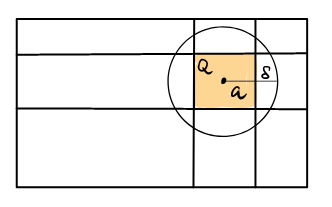
\includegraphics[width=0.4\linewidth]{./images/analisi_complessa/rectangles-singularity-integration.png}
		\caption{}
		\label{fig:rectangles-singularity-integration}
	\end{figure}
	Applicando il teorema di Goursat \ref{thr:groursat} agli otto rettangoli si ottiene che l'integrale sul bordo coincide con l'integrale sul bordo di $Q$. 
	Per ipotesi di $f$ tale che $(z-a_i)f(z) \to 0$ per $z \to a_i$, equivale a dire che per ogni $\varepsilon > 0$ esiste $\delta$ tale che se $|z - a| < \delta$ allora $f(z)(z-a) < \varepsilon$. In particolare poiché la suddivisione fatta può essere arbitraria, ovvero il lato del quadrato $Q$ possiamo sceglierlo in modo tale che per ogni $q\in Q$ vale $|q-a_i| < \delta$, per cui
	\begin{equation*}
	\begin{aligned}
	\left|\int_{\partial Q} f(z)\ dz\right| \le 4 \mathcal{H}^1(\partial Q) \max \frac{\varepsilon }{|z-a_i|} = 8\varepsilon 
	\end{aligned}
	\end{equation*}
	e per l'arbitrarietà di $\varepsilon$ segue la tesi.
\end{proof}

\begin{corollary}
	Sia $f \in \mathcal{O}(\D \setminus \{a_1, \dots, a_n\})$ tale che
	\begin{equation*}
	\begin{aligned}
	\lim_{z\to a_i} (z-a_i)f(z) = 0
	\end{aligned}
	\end{equation*}
	per ogni $i \in \{1, \dots, n\}$. Sia $\gamma$ una curva chiusa con supporto contenuto in $\D \setminus  \{a_1, \dots, a_n\}$ vale
	\begin{equation*}
	\begin{aligned}
	\int_{\gamma} f(z)\ dz = 0
	\end{aligned}
	\end{equation*}
\end{corollary}
\begin{proof}
	Si procede in maniera analoga a quanto visto per il Teorema di Cauchy \ref{thr:cauchy-integrale} per costruire una primitiva di $f$, denotiamola $F$ (questo è possibile grazie al Teorema \ref{thr:goursat-con-singolarità}). Utilizzando le curve opportune (ovvero quelle soddisfacenti le ipotesi), si ottiene la tesi.
\end{proof}

\chapter{Indice e formula integrale di Cauchy}

\begin{definition}
  \label{def:indice-in-z}
  Sia $\morphism{\gamma}{\left[ a,b \right]}{\C}$ una curva chiusa e sia
  $\Omega = \C \setminus \image(\gamma)$. Allora si dice \textbf{indice} di
  $z \in \Omega$ rispetto a $\gamma$ il numero 
  \begin{equation*}
    \Ind_\gamma(z) := \frac{1}{2i\pi} \int_\gamma
    \frac{dw}{w-z}
  \end{equation*}
\end{definition}

\begin{lemma}
  Sia $\morphism{\gamma}{\left[ a,b \right]}{\C}$ una curva chiusa e sia
  $\Omega = \C \setminus \image(\gamma)$. Dato $\Ind_\gamma(z)$
  l'indice di $z \in \Omega$ rispetto a $\gamma$. Allora
  $\Ind_\gamma(z) \in \Z$.
  \label{lem:index-is-natural-number}
\end{lemma}
\begin{proof}
  Definiamo 
  \begin{equation*}
    g(s) := \int^{s}_{a} \frac{\gamma'(t)}{\gamma(t) - z} \ dt
  \end{equation*}
  per cui $g(b) = 2i\pi\Ind_\gamma(z)$ da cui vale che
  $\Ind_\gamma(z) \in \Z$ sse $e^{g(b)} = 1$. 
  
  Diamo un nome a questa funzione $\varphi(s) = e^{g(s)}$. Allora vediamo
  che derivando $\varphi'(s) = \varphi(s) \frac{\gamma'(s)}{\gamma(z) - z}$.
  Da cui si ottiene facilmente che la seguente funzione è costante
  \begin{equation*}
    \left(\frac{\varphi}{\gamma - z}\right)' = 0
  \end{equation*}

  Poiché $\varphi/(\gamma - z)$ è costante e $\gamma(b) = \gamma(a)$ vale 
  \begin{equation*}
    \frac{\varphi(b)}{\gamma(b) - z} = \frac{\varphi(a)}{\gamma(a) - z}
    \Longleftrightarrow \varphi(b) = \varphi(a)
  \end{equation*}
  per cui essendo che $\varphi(a) = e^0 = 1$ vale la tesi.
\end{proof}

\begin{lemma}
  Sia $\Omega \subset \C$ aperto, e $\gamma$ una curva chiusa tale che
  $\image(\gamma) \subset \Omega$ e sia $\morphism{g}{\Omega}{\C}$ una
  funzione continua sul supporto di $\gamma$. Allora la funzione
  \begin{equation*}
    f(z) := \int_\gamma \frac{g(w)}{w-z}\ dw
  \end{equation*}
  è olomorfa su $\C \setminus \image(\gamma)$. 
  \label{lem:index-function-holomorphic}
\end{lemma}
\begin{proof}
  Dimostro che $f$ è continua. Per cui provo a fare una stima puntuale per
  determinare la continuità. Allora sia $z_0 \in \C \setminus
  \image(\gamma)$ e sia $\delta = \dist{z_0}{\image(\gamma)}$. 
  Sia $z \in B_{z_0} (\delta/2)$ allora $|z-\gamma(t)| > \delta/2$ per ogni
  $t$. Quindi
  \begin{align*}
    |f(z) - f(z_0)| & = \left|\int_\gamma \frac{g(w)}{w-z} - 
                         \frac{g(w)}{w - z_0} \right| \\
                         & \le \max_{t}
                         \left|\frac{g(\gamma(t))}{(\gamma(t)-z)(\gamma(t)
                           - z_0}\right| |z-z_0| \mathcal{H}^1(\gamma) \\
                           & \le \frac{2}{\delta}\frac{1}{\delta} |z-z_0|
                           \mathcal{H}^1(\gamma) \max_{\gamma} |g(w)|
  \end{align*}
  e quindi questa quantità converge a $0$ per $z\to z_0$.\\

  Dimostro che $f$ è olomorfa. Fisso un $z_0 \in \C \setminus \image(\gamma)$
  e definisco il rapporto incrementale  
  \begin{equation*}
    r(z) := \frac{f(z) - f(z_0)}{z-z_0} = \int_\gamma
    \frac{g(w)}{(w-z)(w-z_0)}\ dw 
  \end{equation*}
  per quanto dimostrato prima $g(w)/(w-z)$ è una funzione su continua
  $\gamma$e $1/(w - z_0)$ pure (dato che $z_0 \notin \image(\gamma)$.
  Pertanto sappiamo che l'integrale di una funzione continua è continua,
  da cui esiste il limite di $r(z) \to r(z_0)$ per $z \to z_0$. Da cui segue
  che $f$ è olomorfa.
\end{proof}

\begin{corollary}
  La funzione $\Ind_\gamma(z)$ è costante su $\Omega
  \setminus \image(\gamma)$.
  \label{cor:ind-is-constant-over-connex-spaces}
\end{corollary}
\begin{proof}
  Poiché assume solo valori discreti e dev'essere continua per i lemmi
  precedenti, segue che dev'essere costante.
\end{proof}

\begin{corollary}
  Vale $\Ind_\gamma(z) = 0$ per ogni $z$ nella componente
  illimitata di $\C \setminus \image(\gamma)$.  
  \label{cor:index-is-trivial-in-illimited-connex-component}
\end{corollary}
\begin{proof}
  Sia $\image(\gamma) \subset B(0, R)$ ovvero è limitato da una palla di
  raggio $R$. Dato $\varepsilon > 0$ allora possiamo trovare una $z$ tale da
  avere modulo $|z|$ abbastanza grande per cui valga
  \begin{equation*}
    \frac{1}{|w-z|} \le \frac{1}{|z| - |w|} \le \frac{1}{|z| - R}
    < \varepsilon
  \end{equation*}
  per ogni $w \in \image(\gamma)$. Per cui possiamo stimare l'indice di
  $\gamma$ in un punto $z$ esterno alla palla. Per cui
  \begin{equation*}
    |\Ind_\gamma(z)| < \frac{1}{2\pi} \varepsilon
    \mathcal{H}^1(\gamma)
  \end{equation*}
  Ma essendo $\Ind_\gamma(z)$ una funzione costante sulle
  componenti connessere segue che dev'essere $0$ dato che per ogni
  $\varepsilon > 0$ può essere scelto $z$ tale che valga la relazione.
\end{proof}

\begin{remark}
    Questa osservazione è dettata dal fatto che abbiamo definito un entità
    astratta senza argomentare nemmeno per un attimo il suo significato
    geometrico. Infatti l'indice di una curva chiusa $\gamma$ ha un significato
    molto interessante. L'indice rappresenta quante volte la curva si
    \textit{arrotola attorno a una delle componenti connesse che involge} (infatti
    in inglese si usa il termine \textit{winding-numbers}). Cioè un
    cerchio rappresentato dalla curva 
    \begin{equation*}
        f(t) = e^{2i\pi t}
    \end{equation*}
    con $t \in \left[0, 1 \right]$ avvolge la sua \textit{parte interna} una sola
    volta. Infatti $\Ind_f(z) = 1$ per ogni $z \in \D^2 
    \setminus \S^1$.
    \label{rmk:winding-numbers-interpretation}
\end{remark}

\begin{theorem}[Formula integrale di Cauchy]
    Sia $D$ un disco aperto e $f \in \mathcal{O}(D)$ e $\gamma$ una curva
    chiusa con $\image(\gamma) \subset D$. Allora
    \begin{equation*}
        f(z) \Ind_\gamma(z) = \frac{1}{2i\pi} \int_\gamma
        \frac{f(w)}{w-z} \ dw
    \end{equation*}
    per ogni $z \in D \setminus \image(\gamma)$.
    \label{thr:formula-integrale-cauchy}
\end{theorem}
\begin{proof}
  Sia $z \in D \setminus \image(\gamma)$ fissato e sia $g(w) = (f(w) - f(z))
  / (w-z)$ per ogni $w \in D \setminus \left\{ z \right\}$. 
  Allora $g$ è olomorfa su $D \setminus \left\{ z \right\}$ e inoltre vale
  \begin{equation*}
    \lim_{w \to z} g(w) (w-z) = 0
  \end{equation*}
  per la continuità di $f$. Per il Teorema dell'integrale nullo
  \ref{thr:goursat-con-singolarità} (in particolare il corollario 
  al teorema) applicato a $g$ si ha
  \begin{equation*}
    0  = \int_\gamma g(w)\ dw = \int_\gamma \frac{f(w)}{w-z}\ dw
    - f(z)\int_\gamma \frac{dw}{w-z}\ dw 
  \end{equation*}
  da cui segue la tesi.
\end{proof} 

\begin{remark}
  % TODO: Se trovo una dimostrazione carina, lo metto come teorema.
  % Allora: 
  % 1. Dimostrare che separa in due sole componenti connesse.
  % 2. Dimostrare che se hai una curva chiusa, nella sua parte interna
  % hai che |Ind_\gamma(z)| > 0. (lemma a parte) 
  % 3. Da questo poi trovare che dev'essere almeno Ind_\gamma(z) >= 1 
  % o Ind_\gamma(z) <= -1, poi proseguire per ridurre il bound a 
  % Ind_\gamma(z) < 2 e analogamente Ind_\gamma(z) > -2.
  Data una \textbf{curva di Jordan} ovvero una curva regolare a tratti,
  chiusa e semplice (ovvero è iniettiva), allora per il \textbf{teorema
  della curva di Jordan} vale che divide $\C$ in due componenti connesse, 
  una illimitata e una limitata. In particolare se $\gamma$ è orientata 
  positivamente avrà $\Ind_\gamma(z) = 1$ per ogni $z$ nella
  componente connessa limitata, altrimenti sarà orientata negativamente
  e allora $\Ind_\gamma(z) = -1$.
    \label{rmk:teorema-curva-di-jordan}
\end{remark}

\begin{corollary}
    Se $\gamma$ è una curva chiusa di Jordan e $f$ una funzione olomorfa, allora
    per ogni punto interno $z$ vale 
    \begin{equation*}
        f(z) = \frac{1}{2i\pi} \int_\gamma\frac{f(w)}{w-z}\ dw
    \end{equation*}
    \label{cor:curva-jordan-integral-calculation}
\end{corollary}

\begin{corollary}
    Sia $\morphism{f}{\D}{\C}$ una funzione olomorfa e sia $B_a(r) \subset
    \D$ un disco aperto, allora
    \begin{equation*}
        f(a) = \frac{1}{2\pi} \int_0^{2\pi} f(a + re^{it}) \ dt 
    \end{equation*}
    \label{cor:media-integrale}
\end{corollary}
\begin{proof}
  Ovvio per definizione di circonferenza $\gamma(t) = a + re^{it}$ con $t \in
    \left[ 0, 2\pi \right]$. 
\end{proof}
\begin{remark}
    Si può osservare che ponendo $f = u + iv$ il Corollario
    \ref{cor:media-integrale} da la media integrale delle funzioni $u, v$
    sulla circonferenza.
\end{remark}

\section{Applicazioni della formula integrale}

\begin{definition}
  Data $\morphism{f}{\Omega}{\C}$ funzione olomorfa su $\Omega \setminus
  \left\{ a \right\}$, si dice che $a$ è una \textbf{signolarità
  eliminabile} se $\lim_{z\to a} (z-a) f(z) = 0$.
\end{definition}

\begin{theorem}[Distruzione delle singolarità eliminabili]
    Sia $\morphism{f}{\Omega}{\C}$ una funzione olomorfa su $\Omega
    \setminus \left\{ a \right\}$ tale da avere una singolarità eliminabile
    in $a$. Allora esiste $\morphism{\tilde{f}}{\Omega}{\C}$ tale che 
    $\tilde{f}|_{\Omega \setminus \left\{ a \right\}} = f$ e $\tilde{f}$ 
    è olomorfa su tutto $\Omega$.  
  \label{thr:distruzione-singolarita-semplici}
\end{theorem}
\begin{proof}
  Fissiamo una palla attorno alla singolarità eliminabile $a$ di raggio $r$,
  $B_a(r)$. Allora definiamo $\gamma = \partial B_a(r)$. Per il Teorema
  integrale di Cauchy \ref{thr:formula-integrale-cauchy} allora vale 
  \begin{equation*}
    f(z) = \frac{1}{2i\pi} \int_\gamma \frac{f(w)}{w-z}\ dw
  \end{equation*}
  che vale ovunque per ogni $z \in \Omega \setminus \{a\}$. Definiamo
  l'equazione 
  \begin{equation*}
    g(z) =  \frac{1}{2i\pi} \int_\gamma \frac{f(w)}{w-z}\ dw
  \end{equation*}
  su ogni $z \in B_a(r)$ la funzione è olomorfa per Lemma
  \ref{lem:index-function-holomorphic}. Quindi posso definire la seguente
  funzione che sarà olomorfa ovunque su $\Omega$:
  \begin{equation*}
    \tilde{f}(z) := \begin{cases}
      f(z) & z \in \Omega \setminus \left\{ a \right\} \\
      g(z) & \text{altrimenti}
    \end{cases}
  \end{equation*}
\end{proof}

\begin{theorem}[Teorema di Weierstrass]
    Sia $\Omega \subset \C$ aperto e $f \in \mathcal{O}(\Omega)$ con $z_0 \in
    \Omega$ se $\overline{B_{z_0}(r)} \subset \Omega$ allora per ogni $z \in
    B_{z_0}(r)$ vale
    \begin{equation*}
      \begin{aligned}
         f(z) & = \sum^{+\infty}_{n=0} a_n(z-z_0)^n \\ 
         a_n  & =\frac{1}{2i\pi} \int_\gamma \frac{f(w)}{(w-z_0)^{n+1}}\ dw
      \end{aligned}
    \end{equation*}
    dove $\gamma = \partial B_{z_0}(r)$
    \label{thr:weierstrass-analitic-local-form}
\end{theorem}
\begin{proof}
    La dimostrazione è un semplice calcolo con un twist. 
    Prendiamo $z_0 \in \Omega$ e vogliamo calcolare $f(z)$ dove $z\in
    \Omega$. Per la formula integrale di Cauchy vale (ponendo $\gamma
    = \partial B_{z_0}(r)$) 
    \begin{align*}
      f(z) & = \frac{1}{2i\pi} \int_\gamma \frac{f(w)}{w-z}\ dw \\
           & = \frac{1}{2i\pi} \int_\gamma \frac{f(w)}{(w-z_0) - (z-z_0)}\
           dw \\
           & = \frac{1}{2i\pi} \int_\gamma \frac{f(w)}{(w-z_0)}
           \frac{1}{1 - \frac{z - z_0}{w-z_0}} \ dw \\
    \end{align*}
    ma osserviamo che il secondo termine della moltiplicazione non
    è nient'altro che la serie geometrica per cui 
    \begin{align*}
      f(z) 	& = \frac{1}{2i\pi} \int_\gamma \frac{f(w)}{w-z_0}\sum^{+\infty}_{n=0} \left(\frac{z-z_0}{w-z_0}\right)^n \ dw \\
     	 	 	&  = \sum^{+\infty}_{n=0} \left(\frac{1}{2i\pi} \int_\gamma \left(\frac{f(w)}{(w-z_0)}\right)^{n+1} \ dw\right) (z-z_0)^n  \\
    \end{align*}
    poiché la serie converge (si usi ad esempio l'M-test di Weierstrass)
    possiamo spostare la sommatoria dentro e fuori dall'integrale. Da cui
    la tesi.
\end{proof}

\begin{corollary}
  Sia $f \in \mathcal{O}(\Omega)$ allora $f \in C^{\infty}(\Omega)$.
  \label{cor:olomorphism-c-infty}
\end{corollary}
\begin{proof}
  Segue dal Teorema \ref{thr:weierstrass-analitic-local-form}, infatti
  sapendo che derivando la serie si ottiene ancora una serie convergente
  uniformemente, deve essere convergente su tutto $\Omega$ per il Teorema di
  Abel e quindi qualsiasi derivata è convergente uniformemente su tutto
  $\Omega$. 
\end{proof}

\begin{corollary}
  Se $f \in \mathcal{O}(\Omega)$ esistono le derivate complesse $n$-esime
  $f^{n}(z)$ per ogni $z \in \Omega$ e $n \in \N$. Inoltre se
  $\overline{B_{z_0}(r)} \subset \Omega$ e $\gamma = \partial B_{z_0}(r)$
  allora
  \begin{equation*}
    f^n(z_0) = \frac{n!}{2i\pi} \int_\gamma \frac{f(w)}{(w-z_0)^{n+1}}\ dw
  \end{equation*}
\end{corollary}
\begin{proof}
  Essendo $f$ localmente analitica e derivando la serie in $z_0$ si ottiene 
  \begin{equation*}
    f^n(z) = n!a_n 
  \end{equation*}
  da cui la tesi.
\end{proof}

\begin{corollary}[Stime di Cauchy]
  Sia $\Omega \subset \C$ aperto e $\morphism{f}{\Omega}{\C}$ funzione
  olomorfa in $\Omega$. Prendiamo $z_0 \in \Omega$, $\overline{B_{z_0}(r)}
  \subset \Omega$, $\gamma = \partial B_{z_0}(r)$ e $M = \max_{\gamma} |f|$
  allora vale la seguente stima
  \begin{equation*}
    |f^{(n)}(z_0)| \le \frac{n!M}{r^n}
  \end{equation*}
  per ogni $n \in \N$.
  \label{cor:stime-cauchy}
\end{corollary}
\begin{proof}
  \begin{equation*}
    |f^{(n)}(z_0)| \le \frac{n! M}{2\pi r^{n+1}} \mathcal{H}^1(\gamma)
    =\frac{n!M}{r^n}
  \end{equation*}
\end{proof}

\begin{definition}
  Una funzione $\morphism{f}{\Omega}{\C}$ si dice \textbf{intera} se è analitica su
  tutto $\Omega$, con $\Omega = \C$. 
\end{definition}

\begin{theorem}[Liouville]
  Sia $f \in \mathcal{O}(\C)$, ovvero è una funzione intera. Se $f$ è limitata, allora
  $f$ è costante.
  \label{thr:liouville}
\end{theorem}
\begin{proof}
  Sia $K = \sup_{\C} |f|$, allora $K < +\infty$ poiché $f$ limitata. Dal 
  Corollario \ref{cor:stime-cauchy} in $z_0 = 0$ si ha 
  \begin{equation*}
    |f^{(n)}(0)| \le \frac{n! K}{r^n}
  \end{equation*}
  per ogni $r > 0$. Quindi portando al limite $r \to 0$ si ottiene
  $f^{\left(n \right)}(0) = 0$ per ogni $n \ge 1$. Quindi
  \begin{equation*}
    f(z) = \sum^{+\infty}_{n=0} \frac{f^{(n)}(0)}{n!} z^n = f(0)
  \end{equation*}
  poiché vale per ogni $z\in \C$, segue che $f$ dev'essere costante.
\end{proof}

\begin{remark}
	Cosa succede se si prova ad usare il Teorema di Liouville in $\R$? 
	Non funziona. Infatti basta consideare la funzione $\sin(x)$ che è 
	analitica ovunque e limitata (su $\R$), ma non è una funzione costante. 
	Inoltre $\sin(x)$ è una funzione intera, ma non è limitata sui complessi
	e infatti non vale il Teorema di Liouville.
\end{remark}

\begin{corollary}
  Sia $f \in \mathcal{O}(\C)$ e $f = u + iv$. Se $u$ oppure $v$ è limitata
  allora $f$ è costante.
  \label{cor:stronger-liouville-constant-function}
\end{corollary}
\begin{proof}
  Consideriamo la funzione $g(z) = e^{f(z)}$. Allora $|g(z)| = e^{u(z)}$ ed
  essendo $u(z)$ limitata anche $|g(z)|$ lo è. Possiamo applicare quindi il
  teorema di Liouville \ref{thr:liouville} e ottenere che $g(z)$ è una
  costante. Per cui $0 = g'(z) = (e^f)' = e^f f'$ poiché $e^f \neq 0$, segue
  che $f' = 0$, per cui $f$ è costante.\\
  
  Se fosse $v$ limitata allora avrei che la funzione $h(z) = e^{-if(z)}$
  avrebbe modulo limitato e per Liouville $h$ sarebbe costante. Per cui
  $-i e^{-if(z)} f'(z) = 0$ per cui $f'(z) = 0$ per ogni $z$ e $f$ sarebbe
  ancora una volta una funzione costante.
\end{proof}

\begin{theorem}[Teorema fondamentale dell'algebra]
  Ogni polinomio non costante $p(z)$ ha una radice $z_0$ tale che $p(z_0)
  = 0$. 
  \label{thr:fondamentale-dell-algebra}
\end{theorem}
\begin{proof}
  Se $p(z)$ non avesse radici allora $f(z) := \frac{1}{p(z)} \in
  \mathcal{O}(\C)$. In particolare $f$ sarebbe una funzione con modulo
  limitato (infatti l'unico modo perché possa essere non limitata è che
  $p(z) \to 0$ per qualche $z$). In particolare possiamo usare il Teorema di
  Liouville \ref{thr:liouville} e ottenre che $f$ è una funzione costante su
  $\C$, ovvero $p(z)$ è un polinomio costante.
\end{proof}

\begin{theorem}[Morera]
  Sia $\Omega \subset \C$ aperto e $f \in C^0(\Omega)$ e tale che 
    \begin{equation*}
      \int_{\partial R} f(z)\ dz = 0 
    \end{equation*}
    per ogni rettangolo $R \subset \Omega$ allora $f \in
    \mathcal{O}(\Omega)$. 
    \label{thr:morera}
\end{theorem}
\begin{proof}
  Per costruzione analoga a quanto fatto nel Teorema
  \ref{thr:cauchy-integrale} si può creare $F$ primitiva di $f$. Ma poiché
  $F \in \mathcal{O}(\Omega)$ allora è anche $C^{\infty}(\Omega)$ e in
  particolare $f \in C^{\infty}(\Omega)$ ovvero è olomorfa. 
\end{proof}

\begin{corollary}
  Sia $\Omega \subset \C$ aperto e $\{f_n\}$ una successione di funzioni
  olomorfe su $\Omega$. Se $\{f_n\} \to f$ uniformemente sui compatti di
  $\Omega$ (una condizione leggermente più debole che richiedere che sia
  convergente uniformemente su tutto $\Omega$) allora $f$ è olomorfa su
  $\Omega$.  
  \label{cor:trasmissione-olomorfismo-successione}
\end{corollary}
\begin{proof}
  Poiché ogni rettangolo $R \subset \Omega$ è un compatto su $\Omega$,
  allora $\{f_n\} \to f$ converge in modo uniforme. Per cui vale
  \begin{equation*}
    \int_{\partial R} f(z)\ dz = \int_{\partial R} \lim_{n\to+\infty}f_n(z)
    \ dz = \lim_{n\to+\infty} \int_{\partial R} f_n(z)\ dz = 0 
  \end{equation*}
  per il teorema di Morera \ref{thr:morera} risulta che $f$ è olomorfa.
\end{proof}

\section{Teoremi integrali di Cauchy}

% TODO: revise at the end
Come abbiamo visto il campo dei complessi dona meraviglie al calcolo degli
integrali di linea e stabilisce una profonda relazione tra integrale, indice
di una curva e la funzione stessa. Vogliamo ora investigare la
possibilità di calcolare una funzione attraverso il suo integrale nella
maggior parte possibile dello spazio $\Omega$. Ovvero cercare di escludere
solamente i punti dove la funzione ha dei poli.

\begin{definition}
    \label{def:catena-di-curve-chiuse}
    Una \textbf{catena} è una somma finita formale 
    \begin{equation*}
      \Gamma = \sum^n_{i=1} m_i \gamma_i
    \end{equation*}
    dove $\gamma_i$ sono curve chiuse distinte e $C^1$ a tratti con
    i coefficienti $m_i \in \Z$. Inoltre il \textbf{supporto di $\Gamma$}
    è tale che 
    \begin{equation*}
      \image(\Gamma) = \bigcup^n_{i=1} \image(\gamma_i)
    \end{equation*}
\end{definition}

\begin{remark}
  Per come è stata definita la catena di curve chiuse (o meglio per come vogliamo
  che agisca), valgono le seguenti proprietà:
  \begin{enumerate}
    \item Date due catene di curve chiuse $\Gamma_1 = \sum^n_{i=1} m_i
      \gamma^1_i$ e $\Gamma_2 = \sum^m_{j=1} n_j \gamma^2_j$ allora la loro
      somma consiste in $\Gamma_1 + \Gamma_2 =  \sum^n_{i=1} m_i
      \gamma^1_i + \sum^m_{j=1} n_j \gamma^2_j$ e i coefficienti $m_i$
      e $u_j$ vengono raccolti se le curve $\gamma^1_i = \gamma^2_j$.
    \item L'integrale lungo una catena si può calcolare come la somma pesata
      degli integrali lungo le rispettive curve chiuse da cui è composta,
      quindi vale 
      \begin{equation*}
        \int_\Gamma f(z)\ dz := \sum^n_{i=1} m_i \int_{\gamma_i} f(z)\ dz
      \end{equation*}
      data una catena $\Gamma = \sum^n_{i=1} m_i\gamma_i$.
    \item Inoltre si può definire l'indice di una catena come la
      combinazione lineare degli indici delle curve chiuse da cui
      è composta, ovvero 
      \begin{equation*}
        \Ind_\Gamma(z) = \sum^n_{i=1} m_i
        \Ind_{\gamma_i}(z)
      \end{equation*}
  \end{enumerate}
  \label{rmk:operazioni-intuitive-per-le-catene-di-curve-chiuse}
\end{remark}


\begin{definition}
  \label{def:omologia-a-zero}
  Sia $\Omega \subset \C$ aperto e $\Gamma$ una catena di curve chiuse tale
  che $\image(\Gamma) \subset \Omega$. Allora si dice che $\Gamma$
  è \textbf{omologa a zero in $\Omega$} se $\Ind_\Gamma(z)
  = 0$ per ogni $z \in \C \setminus \Omega$. 
\end{definition}

\begin{definition}
  \label{def:omologia-tra-catene}
  Sia $\Omega \subset \C$ aperto e $\Gamma_1,\Gamma_2$ catene di curve 
  chiuse tale che $\image{\Gamma_1}, \image{\Gamma_2} \subset \Omega$. 
  Allora si dice che $\Gamma_1$ e $\Gamma_2$ sono \textbf{olomoghe in 
  $\Omega$} se $\Gamma_1 - \Gamma_2 \sim_\Omega 0$, ovvero vale per ogni $z
  \in \C \setminus \Omega$ che $\Ind_{\Gamma_1}(z)
  = \Ind_{\Gamma_2}(z)$.
\end{definition}

\begin{remark}
  Useremo per indicare l'omologia tra due curve la notazione
  $\Gamma_1 \sim_\Omega \Gamma_2$.
  \label{rmk:notazione-omologia-catene}
\end{remark}

\begin{proposition}
    \label{prop:decomposizione-curva-in-catena-con-n-punti}
    Sia $\Omega \subset \C$ un aperto e sia $\gamma$ una catena tale che
    $\gamma \sim_\Omega 0$. Siano $z_1, \dots, z_n$ punti di $\Omega$
    e siano $D_i$ dei cerchi a due a due disgiunti centrati in $z_i$ e tali
    che $D_i \subset \Omega$. Allora se indichiamo con $\gamma_i = \partial
    D_i$ vale su $\Omega' = \Omega \setminus \left\{z_1,\dots, z_n\right\}$ la
    seguente omologia
    \begin{equation*}
      \gamma \sim \sum^m_{i=1} \Ind_\gamma(z_i) \gamma_i
    \end{equation*}
\end{proposition}
\begin{proof}
     Osserviamo innanzitutto che $\C \setminus \Omega' = (\C \setminus
     \Omega) \cup \{z_1, \dots, z_n\}$. Per cui prendiamo $z\in \C \setminus
     \Omega$ allora vale $\Ind_\gamma(z) = 0$ poiché sappiamo
     che è omologa alla curva $0$. Inoltre vale lo stesso per ogni $i
     = 1,\dot, n$ il seguente $\Ind_{\gamma_i}(z) = 0$. 

     Se invece $z = z_j$ per $j \in \{1, \dots, n\}$ allora
     $\Ind_\gamma(z_j) = m_j$ poiché è possibile che siano 
     nella parte interna di $\image(\gamma)$, mentre
     $\Ind_{\gamma_i}(z_j) = \delta_{i,j}$ ovvero il delta di
     Kronecker. Per cui 
     \begin{equation*}
       \Ind_{\sum^n_{i=1} m_i \gamma_i}(z_j) = m_j
       = \Ind_\gamma(z_j) 
     \end{equation*}
    da cui la tesi.
 \end{proof}

 \begin{lemma}
   Sia $\Omega \subset \C$ un aperto e $f \in \mathcal{O}(\Omega)$
   e $\morphism{g}{\Omega\times\Omega}{\C}$ definita come 
   \begin{equation*}
     g(z,w) :=
     \begin{cases}
       \frac{f(w) - f(z)}{w-z} & w \neq z \\
       f'(z)                   & w = z
     \end{cases}
   \end{equation*}
   è una funzione continua. Inoltre per ogni $w_0 \in \Omega$ fissato vale
   $g(z,w_0) \in \mathcal{O}(\Omega)$.
   \label{lem:rapporto-incrementale-funzione-olomorfa}
 \end{lemma}
 \begin{proof}
    \textbf{Dimostrazione che $g$ è continua} \\
    
    Se $(z_0, w_0) \in \Omega\times\Omega$ con $z_0 \neq w_0$ la
    continuità di $g$ discende dalla definizione dato che il denominatore
    $w_0 - z_0 \neq 0$ e $f$ è olomorfa. 
    Per cui sia $(z_0, z_0) \in \Omega \times \Omega$. Sappiamo che $f'$
    è continua dato che $f$ olomorfa. Per ogni $\varepsilon > 0$ esiste $\delta
    >0$ tale che $|f'(\alpha) - f'(z_0)| \le \varepsilon$ se $\alpha \in
    B_{z_0}(\delta) \subset \Omega$. Quindi fissiamo due punti all'interno
    della palla di raggio $\delta$ e centro $z_0$, ovvero $z,w \in
    B_{z_0}(\delta)$. Allora se $z = w$ si ha 
    \begin{equation*}
      |g(z,z) - g(z_0,z_0)| = |f'(z) - f'(z_0)| \le \varepsilon
    \end{equation*}
    e quindi è continua. Se $z \neq w$ allora
    \begin{align*}
    g(z,w) - g(z_0, z_0) & = \frac{1}{w-z}(f(w) - f(z)) - f'(z_0) \\
    & = \frac{1}{w-z}(f(w)- f(z) - f'(z_0)) 
    \end{align*}
    possiamo definire quindi una retta $\morphism{\gamma}{\left[0,1
    \right]}{\C}$ che unisce i due punti $w$ e $z$ tale che 
    $\gamma(0) = z$ e $\gamma(1) = w$. Quindi $\gamma(t) = (1-t)z+ tw$
    e inoltre $\gamma'(t) = w - z$. Allora possiamo esprimere la formula di
    prima come
    \begin{align*}
       g(z,w) - g(z_0, z_0) & = \frac{1}{w-z}(f(w)- f(z) - f'(z_0)) \\
        & = \frac{1}{w-z} \int_\gamma f'(\alpha) - f'(z_0)\ d\alpha \\
        & = \frac{1}{w-z} \int^1_0 (f'(\gamma(t)) - f'(z_0)) \gamma'(t)\
        dt \\
        & = \int^1_0 f'(\gamma(t)) - f'(z_0)\ dt
    \end{align*}
    da cui si può maggiorare in valore assoluto l'espressione, sapendo
    che per ogni $\varepsilon > 0$ fissato un $\delta >0$ e $z,w \in
    B_{z_0}(\delta)$, con la seguente
    \begin{equation*}
      |g(z,w) - g(z_0,z)| \le \int^1_0 |f'(\gamma(t)) - f'(z_0)|\ dt \le
      \int^1_0 \varepsilon\ dt = \varepsilon
    \end{equation*}
    ovvero $g$ è continua.

   \textbf{Dimostrazione che $g$ è olomorfa dato un $w_0$} \\

   Se $w_0 \in \Omega$ viene fissato, allora $g(z, w_0) \in
   \mathcal{O}(\Omega\setminus\left\{ w_0 \right\})$. Inoltre se $z = w_0$
   è una singolarità eliminamil per $g(z,w_0)$. Per la continuità $g(z,w_0)$
   coincide con la sua estensione olomorfa su tutto $\Omega$ (teorema di
     Distruzione della singolarità eliminabile
   \ref{thr:distruzione-singolarita-semplici}).
 \end{proof}

\begin{theorem}
Sia $\Omega \subset \C$ un aperto e $\Gamma$ una catena in $\Omega$ con
$\Gamma \sim_\Omega 0$. Sia $f \in \mathcal{\Omega}$. Allora 
\begin{enumerate}
    \item Vale la formula integrale di Cauchy per ogni $z \in \Omega \setminus
        \image(\Gamma)$  
        \begin{equation*}
            f(z) \Ind_\Gamma(z) = \frac{1}{2\pi i} \int_\Gamma
            \frac{f(w)}{w-z}\ dw
        \end{equation*}
    \item Vale il teorema dell'integrale nullo di Cauchy 
        \begin{equation*}
            \int_\Gamma f(z) \ dz = 0
        \end{equation*}
\end{enumerate}
\label{thr:formule-di-cauchy-generale}
\end{theorem}
\begin{proof}[1]

    \textbf{Definizioni preliminari}\\

    Sia $\morphism{g}{\Omega\times\Omega}{\C}$ definita come nel Lemma
    \ref{lem:rapporto-incrementale-funzione-olomorfa}. 
    % TODO
    Poniamo quindi 
    \begin{equation*}
        \Omega' := \left\{ z \in \C \setminus \image(\Gamma) \mid
            \Ind_\Gamma(z) = 0  \right\}
    \end{equation*}
    ovvero $\Omega'$ rappresenta la componente connessa esterna alla catena
    $\Gamma$ e quindi è un aperto. % TODO: why?
    Essendo inoltre $\Gamma \sim_\Omega 0$, dev'essere che $\Omega' \supset
    \C \setminus \Omega$.  Per cui $\Omega \cup \Omega' = \C$. Poniamo 
    \begin{equation*}
      h(z) = \begin{cases}
        \frac{1}{2\pi i} \int_\Gamma g(z,w)\ dw  & \text{per} z \in \Omega \\
        \frac{1}{2\pi i} \int_\Gamma \frac{f(w)}{w-z}\ dw \ & \text{per}
        z \in \Omega' 
      \end{cases}
    \end{equation*}
    osserviamo che la definizione è ben posta dato che se $z \in \Omega \cap
    \Omega'$ allora la definizione coincide
    \begin{equation*}
      \frac{1}{2\pi i} \int_\Gamma g(z,w)\ dw =  
            \frac{1}{2\pi i} \int_\Gamma \frac{f(w)}{w-z}\ dw - 
            \frac{f(z)}{2\pi i} \Ind_\Gamma(z) 
            = \frac{1}{2\pi i} \int_\Gamma \frac{f(w)}{w-z}\ dw        
    \end{equation*}
    poiché essendo in $\Omega'$, sappiamo che $\Ind_\Gamma(z)
    = 0$. 
    
    \textbf{Dimostriamo che $h$ è intera}\\

    Osserviamo che $h \in \mathcal{O}(\C)$, infatti $h \in
    \mathcal{O}(\Omega')$ per il Lemma \ref{lem:index-function-holomorphic}
    e inoltre possiamo dimostrare che $h \in \mathcal{O}(\Omega)$ come
    conseguenza del Teorema di Morera \ref{thr:morera}. 
    Bisogna quindi verificare che per ogni disco aperto $D$ tale che anche 
    $\overline{D}\subset \Omega$ e $R \subset D$ è un rettangolo questo si
    annulli. Calcoliamo l'integrale di $h$ lungo $\partial R$ ovvero 
    \begin{equation*}
      \int_{\partial R} h(z)\ dz = \frac{1}{2\pi i} \int_{\partial
      R}\int_\Gamma g(z,w)\ dw\ dz = \frac{1}{2\pi i} \int_\Gamma
      \int_{\partial R} g(z,w) dz\ dw
    \end{equation*}
    per il Teorema di Fubini grazie alla proprietà che $g$ è continua (Lemma
    \ref{lem:rapporto-incrementale-funzione-olomorfa}). Ma sappiamo che 
    \begin{equation*}
      \int_{\partial R} g(z,w) \ dz = 0  
    \end{equation*}
    per ogni $w$ dato che $z \mapsto g(z,w)$ è una funzione olomorfa. Per
    cui segue che $h \in \mathcal{O}(D)$ per ogni disco aperto $D \subset
    \Omega$, per cui è olomorfa su tutto $\Omega$.

    \textbf{Conclusione}\\

    Dobbiamo far vedere che $h$ sia limitata. Prendiamo $z$ abbastanza
    grande e tale che $|z| - |w| > 0$ per ogni $w \in \image(\Gamma)$
    e $\Ind_\Gamma(z) = 0$. Allora $z \in \Omega'$ e vale la
    seguente disuguaglianza
    \begin{equation*}
      2\pi |h(z)| = \left|\int_\Gamma \frac{f(w)}{w-z}\ dz \right| \le
      \left( \sup_{w \in \image(\Gamma)} \frac{|f(w)|}{|z|-|w|} \right)
        \mathcal{H}^1(\Gamma) \overset{|z|\to+\infty}{\to} 0
    \end{equation*}
    Se $|h(z)| \le 1$ per $|z| \ge M$ allora 
    \begin{equation*}
      |h(z)| \le \max \left\{1,\max_{|w| \le M} |h(w)|\right\}
    \end{equation*}
    per ogni $z \in \C$. Quindi per il teorema di Liouville
    \ref{thr:liouville} e poiché il limite a inifinito tende a $0$
    dev'essere che $h(z) = 0$ per ogni $z \in \C$. Per cui segue la tesi, 
    per ogni $z \in \Omega \setminus \image(\Gamma)$ vale 
    \begin{equation*}
      0 = h(z) = \frac{1}{2 \pi i} \int_\Gamma \frac{f(w)}{w-z}\ dw - f(z)
      \Ind_\Gamma(z)  
    \end{equation*}
\end{proof}
\begin{proof}[2]
  Sia $z_0 \in \Omega \setminus \image(\Gamma)$. Per il punto precedente
    applicato alla funzione $F(z) = f(z)(z-z_0)$ vale
    \begin{equation*}
      0 = F(z_0)\Ind_\Gamma(z_0) = \frac{1}{2 \pi i}
      \int_\Gamma f(w)\ dw
    \end{equation*}
\end{proof}

\begin{corollary}
  Se $\Gamma_1 \sim_\Omega \Gamma_2$ allora vale
  \begin{equation*}
    \int_{\Gamma_1}f(z) \ dz = \int_{\Gamma_2 } f(z)\ dz
  \end{equation*}
  \label{cor:uguaglianza-catene-per-integrali}
\end{corollary}

\section{L'indice rispetto alle curve continue}

\begin{lemma}
    Siano $\gamma_1, \gamma_2$ curve chiuse di classe $C^1$ a tratti definite su
    $\left[ a,b \right]$ tali che $z \notin \image{\gamma_1} \cup
    \image{\gamma_2}$. Se vale inoltre che 
    \begin{equation*}
        |\gamma_1(t) - \gamma_2(t)| \le |\gamma_2(t) -z| \quad \text{per
        ogni}\ t \in \left[ a,b \right]
    \end{equation*}
    allora $\Ind_{\gamma_1}(z)
    = \Ind_{\gamma_2}(z)$
    \label{lem:stesso-indice-curve-vicine-in-punto}
\end{lemma}
\begin{proof}
 Dalla definizione segue che $\Ind_\gamma(z)
 = \Ind_{\gamma - z}(o)$. % TODO: perché vale questa cosa?
 % Riguarda la definizione di catena di curve chiuse forse?? 
 Assumiamo quindi $z = 0$. Sia 
 \begin{equation*}
   \gamma(t) = \frac{\gamma_1(t)}{\gamma_2(t)}
 \end{equation*}
 allora vale che $|\gamma(t) - 1| \le 1$ per ogni $t$, inoltre segue dalle
 ipotesi che $z=0 \notin \image(\gamma)$. Dunque $\image(\gamma) \subset
 B_{1}(1)$ e dunque l'origine appartiene alla componente illimitata di $\C
 \setminus \image(\gamma)$, da cui segue per Corollario
 \ref{cor:index-is-trivial-in-illimited-connex-component} che
 $\Ind_\gamma(0) = 0$. Ma 
 \begin{equation*}
   2\pi i \Ind_\gamma(0) = \int_\gamma \frac{dw}{w} = \int_a^b
   \left( \frac{\gamma'_1(t)}{\gamma_1(t)}
   - \frac{\gamma'_2(t)}{\gamma_2(t)}\right) = 2\pi
   i (\Ind_{\gamma_1}(0) - \Ind_{\gamma_2}(0))
 \end{equation*}
 ovvero la tesi.
\end{proof}

\begin{corollary}
  Sia $\morphism{\gamma}{\left[ a,b \right]}{\C}$ una curva continua chiusa
  con $z \notin \image(\gamma)$. Esiste $\delta > 0$ tale che pper ogni
  coppia di curve (di classe $C^1$ a tratti)
  $\morphism{\gamma_1,\gamma_2}{\left[ a,b \right]}{\C \setminus\left\{ z
  \right\}}$ tali che $\|\gamma - \gamma_1\|_\infty < \delta$ e $\|\gamma
  - \gamma_2\| < \delta$ si ha $\Ind_{\gamma_1}(z)
= \Ind_{\gamma_2}(z)$
  \label{cor:carabinieri-tra-due-curve-convergenza-indice}
\end{corollary}
\begin{proof}
  Assumiamo ancora $z = 0$. Sia $\delta = \inf |\gamma(t)|$. Allora per ogni
  $t \in \left[ a,b \right]$ vale 
  \begin{equation*}
    |\gamma_1(t) - \gamma_2(t)| \le |\gamma_1(t) - \gamma(t)| + |\gamma(t)
    - \gamma_2(t)| < 2\delta
  \end{equation*}
  e inoltre vale 
  \begin{equation*}
    |\gamma_2(t)| \ge |\gamma(t)| - |\gamma(t) - \gamma_2(t)| \ge
    2\delta
  \end{equation*}
  e per il Lemma \ref{lem:stesso-indice-curve-vicine-in-punto}, si ottiene
  la tesi.
\end{proof}

\begin{remark}
    Osserviamo che il corollario ci permette di definire
    $\Ind_\gamma(z)$ per una curva $\gamma \in C^0(\Omega)$ e non
    per forza $C^1$ a tratti. Dato che si può approssimare qualsiasi funzione
    continua in modo uniforme attraverso delle poligonali $C^1$ a tratti.
    \label{rmk:generalizzazione-indice-curve-chiuse-continue}
\end{remark}

\begin{theorem}
  Sia $\Omega \subset \C$ aperto. Se $\morphism{\gamma_0, \gamma_1}{\left[
  a,b \right]}{\Omega}$ sono curve continue chiuse e omotope in $\Omega$
  allora vale $\gamma_0 \sim_\Omega \gamma_1$.
  \label{thr:omotopia-implica-omologia}
\end{theorem}
\begin{proof}
  Indichiamo con $\morphism{F}{\left[ a,b \right]\times \left[ 0,1
  \right]}{\Omega}$ l'omotopia tra le curve $\gamma_1$ e $\gamma_2$. Allora
  sia $t_0 \in I$ fissato e sia $\delta > 0$ associamo $\gamma_{t_0}(s) 
  = F(s, 0)$. Inoltre sappiamo che $F$ è uniformemente continua poiché
  continua e definita su un compatto. Quindi esiste $\delta' >0$ tale che 
  \begin{equation*}
    |t-t_0| < \delta' \Longrightarrow \|\gamma_t - \gamma_{t_0}\| < \frac{\delta}{2}
  \end{equation*}
  Fissiamo ora un $t_1$ per cui vale $|t_1- t_0| < \delta'$ e denominiamo
  con $\hat{\gamma}_{t_0}, \hat{\gamma}_{t_1}$ curve di classe $C^1$
  a tratti tali che $\|\gamma_{t_i} - \hat{\gamma}_{t_i}\| < \delta/2$ per
  $i = 0,1$. Allora vale 
  \begin{equation*}
    \|\gamma_{t_0} - \hat{\gamma}_{t_1}\| \le \|\gamma_{t_0}
    - \gamma_{t_1}\| + \|\gamma_{t_1} - \hat{\gamma}_{t_1}\| < \delta
  \end{equation*}
  per il Corollario \ref{cor:carabinieri-tra-due-curve-convergenza-indice}
  vale che $\Ind_{\gamma_{t_0}}(z)
  = \Ind_{{\gamma}_1}(z)$. Per cui segue che la funzione $t
  \mapsto \Ind_{\gamma_t}(z)$ è localmente costante e quindi
  continua e a valori interi sull'insieme connesso $\left[ 0,1 \right]$. In
  particolare è costante e quindi vale $\Ind_{\gamma_0}(z)
  = \Ind_{\gamma_1}(z)$ che era quanto si voleva dimostrare.
\end{proof}

\begin{corollary}
  Sia $\Omega \subset \C$ aperto e $f \in \mathcal{O}(\Omega)$. Se
  $\gamma_0, \gamma_1$ sono curve chiuse di classe $C^1$ a tratti e omotope
  in $\Omega$ allora 
  \begin{equation*}
    \int_{\gamma_0} f(z)\ dz =  \int_{\gamma_1} f(z)\ dz
  \end{equation*}
  \label{cor:omotopia-implica-integrali-di-linea-uguali}
\end{corollary}
\begin{proof}
  Omotopia implica l'omologia delle curve, da cui il teorema per formula
  integrale di Cauchy.
\end{proof}

\begin{corollary}
  Sia $\Omega \subset \C$ aperto e $f \in \mathcal{O}(\Omega)$. Se
  $\gamma_0, \gamma_1$ sono curve chiuse di classe $C^1$ a tratti e omotope
  relativamente a $\{0,1\}$ allora 
  \begin{equation*}
    \int_{\gamma_0} f(z)\ dz = \int_{\gamma_1} f(z)\ dz
  \end{equation*}
  \label{cor:omotopia-curve-aperte-implica-integrali-di-linea-uguali}
\end{corollary}
\begin{proof}
  Possiamo definire la curva chiusa $C^1$ a tratti $\gamma = \gamma_0 \circ
  \gamma^{-1}_1$ è omotopa in $\Omega$ al cammino costante
  $c_{\gamma(0)}$ e dunque si ottiene 
  \begin{equation*}
    0 = \int_\gamma f(z)\ dz = \int_{\gamma_0} f(z)\ dz - \int_{\gamma_1}
    f(z)\ dz
  \end{equation*}
  da cui la tesi.
\end{proof}

\section{Applicazioni dell'indice}

\begin{theorem}
    La mappa $\morphism{\Psi}{\pi(\S^1, 1)}{\Z}$ definita come $\Psi(\left[
    \gamma \right]) = \Ind_\gamma(0)$ è un isomorfismo di gruppi
    e in particolare $\pi(\S^1, 1) \simeq \Z$.
    \label{thr:gruppo-fondamentale-della-circonferenza}
\end{theorem}
\begin{proof}
    Osserviamo che se indichiamo con $\circ$ la composizione di due cappi
    $\alpha, \beta$ allora vale che 
    \begin{equation*}
      \Ind_{\alpha \circ \beta}(z)
      = \Ind_\alpha(z) + \Ind_\beta(z) 
    \end{equation*}
    quindi vale che $\Psi$ sia un omomorfismo tra i due gruppi. \\

    Inoltre $\Psi$ è suriettivo poiché vale, definito $\alpha(t)
    = e^{in\pi}$ vale $\Ind_\alpha(z) = n \in \Z$ per ogni $n
    \in \Z$. \\

    Dobbiamo infine dimostrare che sia anche iniettiva. Quindi dobbiamo
    mostrare che $\operatorname{ker}(\Psi) = \{\left[ c \right]\}$. Per cui
    prendiamo una classe $\left[ \alpha \right] \in
    \operatorname{ker}(\Psi)$ e un suo rappresentante
    $\morphism{\gamma}{\left[ 0,1 \right]}{\S^1 \subset \C}$. Poniamo $t
    \in I$ allora definiamo 
    \begin{equation*}
      g(t) := \frac{1}{2\pi i} \int^t_0 \frac{\gamma'(s)}{\gamma(s)}\ ds
      \quad f(t) := e^{2\pi i g(t)}
    \end{equation*}
    la funzione $g$ soddisfa le condizioni $g(0) = g(t)
    = \Ind_\gamma(z) = 0$. Inoltre $g' = \gamma' / (2\pi
    i \gamma)$ e quindi si può riscrivere $f' = f\gamma' / \gamma$. Da
    questa osservazione si può dedurre che $f/\gamma$ è una funzione
    costante dato che 
    \begin{equation*}
      \left(\frac{f}{\gamma}\right)' = \frac{f'}{\gamma}
      - \frac{f\gamma'}{\gamma^2} = 0
    \end{equation*}
    ed essendo che $f(0)/\gamma(0) = 1$ allora vale per ogni $t$. In
    particolare vuol dire che $f = \gamma$ per ogni $t$. Per cui $\gamma(t)
    = e^{2\pi i g(t)}$ e dunque $|\gamma| = 1$ per ogni $t$. 
    Sapendo che quindi $\gamma(t)$ può solo \textit{girare} nella
    circonferenza di raggio $1$ dato che ha modulo costante, dev'essere che 
    $g(t) \in \R$ per ogni $t$, allora è un cappio in $(\R, 0)$. Ma essendo
    $\R$ semplicemente connesso, segue che $g$ è omotopo al cappio
    costante in $0$.
    Pertanto $\gamma$ è omotopo a $e^{2\pi i 0} = 1$. Ovvero per qualsiasi
    rappresentante scelto della classe $\alpha \in \operatorname{ker}(\Psi)$, 
    si ha che la classe $\alpha = \left[c\right]$ ovvero la classe costante. 
\end{proof}

\begin{theorem}
  Sia $\Omega \subset \C$ aperto e semplicemente connesso. Sia $u \in
  C^2(\Omega)$ funzione armonica. Allora esiste $v \in C^2(\Omega)$ tale che
  $f = u + iv$ è olomorfa su $\Omega$.
  \label{thr:esistenza-armonica-congiunta}
\end{theorem}
\begin{proof}
    Osserviamo che $\pi_1(\Omega, z_0) = \{1\}$ dato che è connesso e dato che
    $u$ è armonica abbiamo che definendo $g = u_x - iu_y$ allora $g$ soddisfa le
    condizioni di Cauchy-Riemann, pertanto $g \in \mathcal{O}(\Omega)$. Per il
    Corollario \ref{cor:omotopia-curve-aperte-implica-integrali-di-linea-uguali}
    segue che indipendentemente dalla curva $\gamma$ scelta che unisce $z$
    a $z_0$ vale
    \begin{equation*}
        h(z) := \int_\gamma g(w)\ dw
    \end{equation*}
    ovviamente $h \in \mathcal{O}(\Omega)$ e $h' = g$.
    Quindi descrivendo $h(z) = \alpha(z) + i\beta(z)$ vale che $u_x = \Re(g)
    = \alpha_x$ e $u_y = -\Im(g) = \beta_x = -\alpha_y$. Quindi possiamo
    osservare che $u_x - \alpha_x = 0 = u_y - \alpha_y$ da cui si può
    concludere che la funzione $(u-\alpha)(z) = c \in \C$ è costante e in 
    particolare è una costante reale per come è stata definita $u$, infatti 
    vale $c \in \R$. Per concludere basta osservare che definendo 
    $f = (u - \alpha) + h = u + i\beta$ allora $\Re(f) = u$ e $f \in
    \mathcal{O}(\Omega)$.
\end{proof}




\chapter{Esempi di funzioni complesse}

\section{Funzione esponenziale}

\begin{definition}
	\label{defn:funzione-esponenziale}
	Definiamo l'esponenziale con la serie di potenze
	\begin{equation}
	\begin{aligned}
		e^z := \sum^{+\infty}_{k=0} \frac{z^k}{k!}
	\end{aligned}
	\end{equation}
\end{definition}

Osserviamo alcune proprietà 

\begin{theorem}
	La funzione esponenziale gode delle seguenti proprietà
	\begin{enumerate}
		\item è olomorfa su $\C$.
		\item $(e^z)' = e^z$.
		\item $e^{i\theta} = \cos \theta + i\sin \theta$ per $\theta \in \R$.
		\item è periodica di periodo $2\pi i$.
		\item $e^z \neq 0$ per ogni $z \in \C$. In particolare non è biunivoca.
	\end{enumerate}
\end{theorem}
\begin{proof}[1]
	Per definizione e per il Teorema \ref{thr:teorema-di-abel}.
\end{proof}
\begin{proof}[2]
	Basta un calcolo esplicito della derivata della serie di potenze
	\begin{equation}
	\begin{aligned}
		(e^z)' & = \sum^{+\infty}_{n=1} n\frac{z^{n-1}}{n!} = \sum^{+\infty}_{n=1} \frac{z^{n-1}}{(n-1)!} \\
				& = \sum^{+\infty}_{p=0} \frac{z^p}{p!} = e^z 
	\end{aligned}
	\end{equation}
\end{proof}
\begin{proof}[3]
	Anche per questo basta un calcolo esplicito
	\begin{equation}
	\begin{aligned}
		e^{iz} & = \sum^{+\infty}_{n=0} \frac{(iz)^{n}}{n!} = \sum^{+\infty}_{k=0} \frac{(iz)^{2k}}{2k!} + \sum^{+\infty}_{k=0} \frac{(iz)^{2k+1}}{2k+1!}\\
			& = \sum^{+\infty}_{k=0} (-1)^k\frac{z^{2k}}{2k!} + i\sum^{+\infty}_{k=0} (-1)^k\frac{z^{2k+1}}{2k+1!}\\
			& = \cos z + i \sin z
	\end{aligned}
	\end{equation}
\end{proof}
\begin{proof}[4]
	Basta osservare che $e^{a + 2\pi i} = e^a e^{2\pi i } = e^a$, il fatto che $e^{2\pi i} = 1$ è naturale dal punto precedente.
\end{proof}
\begin{proof}[5]
	Sia $\alpha \in \C$, allora $e^z = \alpha$ vuol dire che se $z = x+iy$ allora 
	\begin{equation}
	\begin{cases}
		x = \ln |\alpha|\\
		y = \arg \alpha
	\end{cases}
	\end{equation}
	per cui se $\alpha = 0$, $x$ non sarebbe ben definito. Mentre per tutti gli altri valore di $\alpha \in \C$ è definita.
\end{proof}

\section{Funzioni trigonometriche}
	
	\begin{definition}
		\label{defn:sin-cos}
		Definiamo le funzioni trigonometriche in funzione delle serie di potenze come segue
		\begin{equation}
		\begin{aligned}
			\sin(z) := \sum^{+\infty}_{k=0} (-1)^k\frac{z^{2k+1}}{(2k+1)!} \;\ \cos(z) := \sum^{+\infty}_{k=0} (-1)^k\frac{z^{2k}}{(2k)!}
		\end{aligned}
		\end{equation}
	\end{definition}
	
	\begin{theorem}
		Valgono i seguenti fatti sulle funzioni trigonometriche
		\begin{enumerate}
			\item 
			\begin{equation}
			\begin{aligned}
				\sin(z) = \frac{e^{iz} - e^{-iz}}{2} \;\ \cos(z) = \frac{e^{iz} + e^{-iz}}{2}
			\end{aligned}
			\end{equation}
			\item sono $2\pi$ periodiche.
			\item non sono limitate.
			\item l'immagine di $\sin$ e $\cos$ coincide con $\C$.
			\item le seguenti funzioni sono olomorfe tranne nei loro rispettivi poli
			\begin{equation}
			\begin{aligned}
				\tan z & := \frac{\sin z}{\cos z} \in \mathcal{O}(\C \setminus \{ \pi /2 + k\pi \mid k \in \N \}) \\
				\cot z & := \frac{\cos z}{\sin z} \in \mathcal{O}(\C \setminus \{k\pi \mid k \in \N \})
			\end{aligned}
			\end{equation}
		\end{enumerate}
	\end{theorem}
	\begin{proof}[1]
		% TODO
	\end{proof}
	\begin{proof}[2]
		% TODO: DIMOSTRAZIONE
	\end{proof}
	\begin{proof}[3]
		% TODO: DIMOSTRAZIONE
	\end{proof}
	\begin{proof}[4]
		% TODO: DIMOSTRAZIONE
	\end{proof}
	\begin{proof}[5]
		% TODO: DIMOSTRAZIONE
	\end{proof}
	
\section{Funzione logaritmo}
	
	\begin{definition}
		\label{defn:logaritmo-principale}
		Il \textbf{logaritmo principale} è la funzione 
		\begin{equation}
		\begin{aligned}	
			\morphism{\log}{\C \setminus \{x \in \R \mid x \le 0\}}{\C}
		\end{aligned}
		\end{equation}
		definita da $\log(z) = \ln(|z|) + i\arg z$ con $\arg z \in \left(-\pi,\pi\right]$ 
	\end{definition}

	\begin{remark}
		In generale si perdono molte delle proprietà del logaritmo sui reali. Per esempio $\log(xy) \neq \log(x)+\log(y)$.
	\end{remark}

	\begin{theorem}
		La funzione logaritmo princiaple è olomorfa e la sua derivata è $\log'(z) = 1/z$.
	\end{theorem}
	\begin{proof}
		Dimostriamo che è olomorfa per le equazioni di Cauchy-Riemann, per cui ponendo
		\begin{equation}
		\begin{aligned}
			\log(x+iy) = \frac{1}{2}\ln(x^2 + y^2) + i\arctan(y/x) = u(x,y) + iv(x,y)
		\end{aligned}
		\end{equation}
		da cui le derivate ci danno le relazioni cercate.\\
		
		Sempre per le equazioni di Cauchy-Riemann otteniamo che $\log(z) = u_x + iv_x = 1/z$.
	\end{proof}
	\begin{remark}
		Osserviamo infine che poiché la funzione argomento può prendere valori con periodicità di $2\pi$, abbiamo effettivamente infinite definizioni della funzione logaritmo. Questo può presentare alcuni vantaggi. Infatti la funzione radice quadrata 
		$f_0(z) = e^{\log(z)/2} = \sqrt{|z|}e^{i(\arg z)/2}$, ma se si usa un'altra definizione di logaritmo, ovvero consideriamo un'altra possibile branca o determinazioni possibili della radice quadrata. Allora otteniamo $f_1(z) = e^{\log'(z)/2} = \sqrt{|z|}e^{i\arg(z)/2 + i\pi}$ che rappresenta la radice `negativa'. E così via per molte altre funzioni.
	\end{remark}

%\appendix
%    Include appendix "chapters" here.
%\include{}

% TODO? bibliografia
%\backmatter
%    Bibliography styles amsplain or harvard are also acceptable.
%\bibliographystyle{amsalpha}
%\bibliography{}
%    See note above about multiple indexes.
\printindex

\end{document}

%-----------------------------------------------------------------------
% End of amsbook-template.tex
%-----------------------------------------------------------------------
